% !TeX root = bbchallenge-paper.tex

\title{Determination of the fifth Busy Beaver value}
\author{
        The bbchallenge Collaboration
}

\documentclass[a4paper,british]{article}

\usepackage{babel}
\usepackage[utf8]{inputenc}
\usepackage[margin=1in]{geometry}
%\usepackage{subfig}
\usepackage[hidelinks]{hyperref}
\usepackage{caption}
\usepackage{floatpag}
\usepackage{subcaption}
\usepackage{tikz}

\usepackage{algorithm}
\usepackage[noend]{algpseudocode}
\usepackage{xcolor,colortbl,tikz}

\usepackage{bold-extra}% bold texttt

\usepackage{graphicx}
\usepackage{mathtools}

\usepackage{booktabs} 

\usepackage{amsmath,amsfonts,amssymb,amsthm}

\theoremstyle{definition} % don't use italics
\newtheorem{theorem}{Theorem}[section]
\newtheorem{definition}{Definition}[section]
\newtheorem{lemma}{Lemma}[section]
\newtheorem{proposition}{Proposition}[section]
\newtheorem{corollary}{Corollary}[section]
\numberwithin{equation}{section}


\theoremstyle{definition} % emphasize the "Remark N." with italics, not bold
\newtheorem{observation}{Observation}[section]
\newtheorem{example}{Example}[section]
\newtheorem{remark}{Remark}[section]

\usepackage{xassoccnt}
\DeclareCoupledCountersGroup{theorems}
\DeclareCoupledCounters[name=theorems]{theorem,definition,lemma,proposition,corollary,remark,observation,example}

\usepackage{microtype,xspace,wrapfig,multicol} 
\usepackage[textsize=tiny,color=lightgray]{todonotes} 
\usepackage[normalem]{ulem} % sout
\usepackage{stmaryrd}


\newcommand{\ts}[1]{{\color{red}#1}}
\newcommand{\tsi}[1]{\todo[inline]{TS: #1}}
\newcommand{\tsm}[1]{\todo{TS: #1}}
\newcommand{\tss}[2]{{\ts{\sout{#1}}} {\ts{#2}}}
\newcommand{\jb}[1]{{\color{blue}#1}}
\newcommand{\jbi}[1]{\todo[inline]{JB: #1}}
\newcommand{\jbm}[1]{\todo{JB: #1}}
\newcommand{\jbs}[2]{{\jb{\sout{#1}}} {\jb{#2}}}
\newcommand{\tabi}{\hspace{\algorithmicindent}}
\newcommand{\Lim}[1]{\raisebox{0.5ex}{\scalebox{0.8}{$\displaystyle \lim_{#1}\;$}}}
\newcommand{\N}{\mathbb{N}}
\newcommand{\Z}{\mathbb{Z}}

\newcommand{\lhead}[1]{\stackrel{#1}\triangleleft}
\newcommand{\rhead}[1]{\stackrel{#1}\triangleright}

\newcommand{\tm}[1]{\href{https://bbchallenge.org/#1}{\nolinkurl{#1}}}

\usepackage{xcolor}

\definecolor{colorA}{RGB}{255,0,0}
\definecolor{colorB}{RGB}{255,128,0}
\definecolor{colorC}{RGB}{0,0,255}
\definecolor{colorD}{RGB}{0,255,0}
\definecolor{colorE}{RGB}{255,0,255}

\newcommand{\stateA}{{\textcolor{colorA}{A}}\xspace}
\newcommand{\stateB}{{\textcolor{colorB}{B}}\xspace}
\newcommand{\stateC}{{\textcolor{colorC}{C}}\xspace}
\newcommand{\stateD}{{\textcolor{colorD}{D}}\xspace}
\newcommand{\stateE}{{\textcolor{colorE}{E}}\xspace}

\newcommand{\szero}{\texttt{0}\xspace}
\newcommand{\sone}{\texttt{1}\xspace}

\def\@fnsymbol#1{\ensuremath{\ifcase#1\or *\or \dagger\or \ddagger\or
   \mathsection\or \mathparagraph\or \|\or **\or \dagger\dagger
   \or \ddagger\ddagger \else\@ctrerr\fi}}
\newcommand{\ssymbol}[1]{^{\@fnsymbol{#1}}}

\newcommand{\BBtheFourth}{107}
\newcommand{\SigmaTheFourth}{13}
\newcommand{\BBtheFourthTNF}{858{,}909}

\newcommand{\BBtheFifth}{47{,}176{,}870}
\newcommand{\BBtheFifthTNF}{181{,}385{,}789}
\newcommand{\SigmaTheFifth}{4{,}098}

\newcommand{\BBTxF}{3{,}932{,}974}
\newcommand{\BBTxFTNF}{2{,}154{,}217}

\newcommand{\radofull}{Tibor Rad\'o\xspace}
\newcommand{\rado}{Rad\'o\xspace}

\newcommand{\cryptid}{Cryptid\xspace}

\newcommand{\cycler}{Cycler\xspace}
\newcommand{\cyclers}{Cyclers\xspace}
\newcommand{\TC}{Translated Cycler\xspace}
\newcommand{\TCs}{Translated Cyclers\xspace}

\newcommand{\headpos}{head-position\xspace}
\newcommand{\headposs}{head-positions\xspace}

\newcommand{\states}{\mathcal{S}}
\newcommand{\alphabet}{\mathcal{A}}
\newcommand{\symbolzero}{\texttt{0}}
\newcommand{\symbolone}{\texttt{1}}

\newcommand{\numSporadic}{13\xspace}

\newcommand{\ssp}{state-symbol-pair\xspace}
\newcommand{\ssps}{state-symbol-pairs\xspace}

\newcommand{\HALT}{\texttt{HALT}\xspace}
\newcommand{\NONHALT}{\texttt{NONHALT}\xspace}
\newcommand{\UNKNOWN}{\texttt{UNKNOWN}\xspace}

\newcommand{\CoqBB}{Coq-BB5\xspace}
\newcommand{\CoqBBnospace}{Coq-BB5}

\newcommand{\TMstep}{\to}

\begin{document}
\date{}
\maketitle

\begin{abstract}
    We prove that $S(5) = 47,176,870$ using the Coq proof assistant. The Busy Beaver value $S(n)$ is the maximum~number of steps a halting n-state 2-symbol Turing machine can perform from the all-0 tape before halting and $S$ was historically introduced by \radofull in 1962 as one of the simplest examples of a noncomputable function.  The proof enumerates 181,385,789 Turing machines with 5 states, and, for each machine, decides whether it halts or not.
    Our result marks the first determination of a new Busy Beaver value in over 40 years and the first Busy Beaver value to ever be formally verified, demonstrating the effectiveness of collaborative online research (\url{bbchallenge.org}).
\end{abstract}


\setcounter{tocdepth}{2}
\tableofcontents

\paragraph{The bbchallenge Collaboration (credits).} The following contributions resulted in the determination of the fifth Busy Beaver value: mxdys (\CoqBB, Loops, RepWL); Nathan Fenner, Georgi Georgiev a.k.a~Skelet, savask (NGramCPS); Justin Blanchard, Mateusz Naściszewski, Konrad Deka (FAR); Iijil (WFAR); mei (\texttt{busycoq}); Shawn Ligocki, Jason Yuen, mei (Sporadic Machines ``Shift Overflow Counters''); Shawn Ligocki, Pavel Kropitz, mei (Sporadic Machine ``Skelet \#1''); Chris Xu, mxdys (Sporadic Machine ``Skelet \#17''); Shawn Ligocki, Dan Briggs, mei (Sporadic Machine ``Skelet \#10''); Justin Blanchard, mei (Sporadic Machines ``Finned Machines''); Yannick Forster (Coq review); Tristan Stérin (bbchallenge.org).
\newpage

\begin{center}

\end{center}



\begin{figure}
    \begin{quote}
        ``In any case, even though skilled mathematicians and experienced programmers attempted to evaluate $\Sigma(3)$ and S(3), there is no evidence that any known approach will yield the answer, even if we avail ourselves of high-speed computers and elaborate programs. As regards $\Sigma(4)$, $S(4)$ the situation seems to be entirely hopeless at present.'' --- \radofull, 1963 \cite{Rado_1963}
    \end{quote}
    \begin{quote}
        ``\textit{Prediction 5}. It will never be proved that $\Sigma(5) = \SigmaTheFifth$ and $S(5) = \BBtheFifth$.'' --- Allen H. Brady, 1990 \cite{BradyMeaningOfLife}
    \end{quote}
    \caption{\radofull, who invented the Busy Beaver game, proved the value of $S(2)$ in 1962 \cite{Rado_1962}, and was involved in the proof of $S(3)$ in 1963 \cite{Lin1963}, did not believe that $S(4)$ could be solved at his time. Allen H. Brady, who proved the value of $S(4)$ in 1983 \cite{Brady83}, did not believe that $S(5)$ could be solved at all. Amusingly, Brady opens his article on $S(4)$ with \rado's above quote \cite{Brady83}. Under that light, the knowledge of a (small) Busy Beaver value seems to be a reflection of the computing technology available at the time it was proved.}
\end{figure}

\vspace{-40pt}

\section{Introduction}

\subsection{Main Results}\label{sec:intro:mainresults}

\newcommand{\noncomput}{noncomputable\xspace}
\newcommand{\BBfull}{Busy Beaver\xspace}
\newcommand{\Coq}{Coq\xspace}
% We'll update this link to v1 release URL
\newcommand{\CoqProofReleaseURL}{\url{https://github.com/ccz181078/Coq-BB5}}

\newcommand{\ie}{i.e.~}
\newcommand{\eg}{e.g.~}

Are there simple \noncomput functions? What is the \textit{smallest} open problem in mathematics? What do algorithms look like, \textit{in the wild}?

Introduced by \radofull in 1962, \textit{the \BBfull game} gives a framework to answer these seemingly independent questions, starting with the first one since \rado's goal was to ``present some very simple instances of \noncomput functions'' \cite{Rado_1962}. The game is as such: (i) run all $n$-state Turing machines\footnote{See Section~\ref{sec:TMs} for Turing machines definitions and examples.} from the all-zero tape (ii) consider the set of machines that eventually halt (iii) the winner of the game is the halting machine that has the most \sone symbols on its tape when it halts. This maximum number of \sone symbols on halting tape among $n$-state machines is called $\Sigma(n)$. \rado also introduced $S(n)$, the maximum number of steps made by a halting $n$-state Turing machine from all-zero tape. Both functions $\Sigma$ and $S$ are \noncomput! This is most obvious in the case of $S$: if an $n$-state machine runs for more than $S(n)+1$ steps, we know it will never halt, giving an algorithm to decide Turing's halting problem if $S$ was computable. This tight link between $S$ and the halting problem makes it more interesting and practical to us than $\Sigma$, hence we take the liberty to concentrate more on $S$.

%This tight link to the halting problem makes $S$ more interesting and practical to us than $\Sigma$, hence we take the liberty (similarly to other authors \cite{BusyBeaverFrontier,otherexamples?}) to focus the busy beaver game on $S$ instead of $\Sigma$ and to call the $n$-state \textit{busy beaver winner} the machine achieving $S(n)$ running steps. 
While there is no algorithm to compute $S(n)$ for \textit{all} $n$ we can certainly try to compute $S(n)$ for \textit{some} $n$. Prior to this work, only the four first values of $S$ had been proved: $S(1)=1$, $S(2)=6$ \cite{Rado_1962}, $S(3) = 21$ \cite{Lin1963}, $S(4) = 107$ \cite{Brady83}. With some early attempts in the 1960s and 1970s, the $S(5)$ quest seriously started in 1983 with a 2-day competition organised at the University of Dortmund\footnote{Report of the competition: \url{https://docs.bbchallenge.org/other/lud20.pdf}.} with the sole goal of finding new 5-state champions -- \ie 5-state machines achieving better $S$ scores than any machines previously known \cite{PMichel_website,michel2019busy}. The winning machine in Dortmund achieved $134,467$ steps, establishing $S(5) \geq 134,467$. In 1989, a big step was made when Marxen and Buntrock found a new champion achieving $\BBtheFifth$ steps \cite{Marxen_1990}, showing $S(5) \geq \BBtheFifth$; this machine is given in Figure~\ref{fig:bb5}. However, it remained unknown if no other machine could beat it, \ie whether Marxen and Buntrock's machine was the actual 5-state Busy Beaver winner or not. In 2020, Aaronson conjectured that there was no better 5-state machine, \ie $S(5) = \BBtheFifth$ \cite{BusyBeaverFrontier}.

Our main result is to prove this conjecture, using the \Coq proof assistant \cite{the_coq_development_team_2024_14542673}, see Theorem~\ref{th:BB5}. The winning machine for $S(5)$ is also the winning machine for $\Sigma(5)$. We also prove $\Sigma(5) = \SigmaTheFifth$, see Theorem~\ref{th:BB5Sigma}.

\begin{theorem}\label{th:BB5}
    $S(5) = \BBtheFifth$.
\end{theorem}

The function $S$ can naturally be extended to Turing machines using more than two alphabet symbols \cite{BradyMeaningOfLife}, like, for instance, $S(2,3) = 38$ is the value of $S$ for 2-state, 3-symbol machines \cite{BradyMeaningOfLife, MICHEL200445, LafittePapazian2007}. We prove, using Coq, that $S(2,4) = \BBTxF$, see Theorem~\ref{th:BB2x4} and Figure~\ref{fig:bb2x4}:

\begin{theorem}\label{th:BB2x4}
    $S(2,4) = \BBTxF$.
\end{theorem}

The Coq proofs for $S(5)$ and $S(2,4)$ --- as well as for previously known $S(2),\,S(3),\,S(4)$ and $S(2,3)$ --- are available at \url{https://github.com/ccz181078/Coq-BB5}. The lists of all the Turing machines evaluated by these proofs are available at \url{https://docs.bbchallenge.org/CoqBB5_release_v1.0.0/}.

The goal of this paper is to present these proofs. As a result of our work, we now have a clearer view of the landscape of small Busy Beaver values, see Table~\ref{table:landscape}.


\setlength{\fboxrule}{1.2pt}
\begin{table}[h]
    \centering
    \small
    \renewcommand{\arraystretch}{1.3}
    \setlength{\tabcolsep}{5pt}  % Adjust column spacing
    \begin{tabular}{c|ccccc}
        \hline
        \textbf{Symbols} & \textbf{2-State}                                                           & \textbf{3-State} & \textbf{4-State} & \textbf{5-State} & \textbf{6-State} \\
        \hline
        2                & \cellcolor{green!20}$S(2) = 6$ \cite{Rado_1962}
                         & \cellcolor{green!20}$S(3) = 21$ \cite{Lin1963}
                         & \cellcolor{green!20}$S(4) = 107$ \cite{Brady83}
                         & \cellcolor{green!50}{$S(5) = \BBtheFifth$}
                         & \cellcolor{orange!50}{$S(6) > 10 \uparrow \uparrow 15$}                                                                                                \\
        \hline
        3                & \cellcolor{green!20}$S(2,3) = 38$ \cite{LafittePapazian2007}
                         & \cellcolor{orange!50}{$S(3,3) > 10^{17}$}
                         & \cellcolor{orange!20}$S(4,3) > 2 \uparrow \uparrow \uparrow 2^{2^{{32}}} $
                         & --                                                                         & --                                                                        \\
        \hline
        4                & \cellcolor{green!50}{$S(2,4) = \BBTxF$}
                         & \cellcolor{orange!20}$S(3,4) > 2 \uparrow^{15} 5 $
                         & --                                                                         & --               & --                                                     \\
        \hline
        5                & \cellcolor{orange!50}{$S(2,5) > 10 \uparrow \uparrow 4$}
                         & --                                                                         & --               & --               & --                                  \\
        \hline
    \end{tabular}
    \caption{Landscape of small busy beaver values.
        \cellcolor{green!20}Cells highlighted in green correspond to values for which we provide \Coq proofs. Bright green indicates the new results, $S(5)$ and $S(2,4)$, original to this work.
        Cells highlighted in orange indicate the existence of a Cryptid (\ie machines whose halting problem is currently open and believed to be mathematically hard), see Appendix~\ref{app:cryptids}. Lighter orange means that the existence of a Cryptid comes trivially from reusing a known 3-state 3-symbol Cryptid and ignoring the available additional state or symbol. }
    \label{table:landscape}
\end{table}











\paragraph{Challenges.} Proving $S(5) = \BBtheFifth$ required analyzing the behavior of $\BBtheFifthTNF$ Turing machines\footnote{This exact number can only be known after the proof is done, see Section~\ref{sec:enum}.}-- evidently requiring computer assistance. The challenge for a halting machine is the case where it halts after a number of steps that is too enormous to be simulated step-by-step (e.g. the current 6-state champion halts after $10 \uparrow \uparrow 15$ steps \cite{Pavel_discorvery}, see Appendix~\ref{app:lowerbounds}), this challenge was not met for 5-state machines since they halt in at most $\BBtheFifth$ steps -- this could not have been known for certain in advance but was believed -- which is easy to simulate on modern computers. The challenge for a non-halting machine is that proving it does not halt can be hard. How hard?

Dauntingly, any $\Pi_1^0$ mathematical statement\footnote{A $\Pi_1^0$ statement is a statement of first-order logic of the form ``$\forall x, \phi(x)$'' where $\phi$ is a sentence with only bounded quantifiers (\ie $\phi(x)$ can always be verified by a computer in finite time).} can be encoded as the halting problem of a Turing machine (from all-zero tape). Such statements are common and include famous open problems in mathematics such as Goldbach's conjecture or the Riemann hypothesis. Goldbach's conjecture, formulated in 1742, is one of the oldest open problems in mathematics and states ``every even positive integer greater than 2 is the sum of two prime numbers.'' We can build a Turing machine that halts iff the conjecture is false: by enumerating all positive integers, then for each, test all sums of smaller primes and halt iff we do not find the sum. A (formally verified) machine performing this procedure has been built using only 25 states \cite{GoldbachTM27, GoldbachTM25}. This means that proving the value of $S(25)$ is at least as hard as solving Goldbach's conjecture because the proof of $S(25)$ must contain an argument as of why this particular 25-state machine does not (or, believed less likely, does) halt. Similarly, the Riemann hypothesis has been encoded in a 744-state machine \cite{RiemannTM,Yedidia2016,BusyBeaverFrontier}. As low as 15 states is enough to encode a hard number theoretical conjecture by Erd\H{o}s \cite{BB15}. Worst, the consistency of common axioms sets such as Peano's Arithmetic (PA) or Zermelo–Fraenkel set theory (ZF) is also $\Pi_1^0$ since one can enumerate proofs in these systems until the proof of a contradiction is found. This has been done for ZF, using 748 states \cite{ZFTM,Yedidia2016,BusyBeaverFrontier,BB748Thesis}. By G\"odel's second incompleteness theorem, this means that proving the value of $S(748)$ cannot be done using ZF. Aaronson conjectures that as low as $S(20)$ cannot be proven in ZF and as low as $S(10)$ cannot be proven in PA \cite{BusyBeaverFrontier}.

Hence, while 5-state halting machines were not feared, it remained unknown how hard non-halting 5-state machines could get. This article settles the question: the smallest open problem in mathematics (on the Busy Beaver scale) does not arise from 5-state machines -- but we have good contenders for 6-state machines, see Section~\ref{sec:cryptids}.

\paragraph{Related Work.} The proof of $S(4) = \BBtheFourth$ was published in 1983 \cite{Brady83}. One of its main innovations was the introduction of a method to solve the halting problem of a category of machines the author calls \textit{XMas Trees}. A caveat of \cite{Brady83} resides in the following quote from the paper: ``All of the remaining holdouts were examined by means of voluminous printouts of their histories along with some program extracted features. It was determined to the author's satisfaction that none of these machines will ever stop.'' A \textit{holdout} is a machine still needing a proof of halting/nonhalting. Using Coq, we bring additional confirmation that $S(4) = \BBtheFourth$, see Theorem~\ref{th:BB4}.

\newcommand{\SkeletHoldoutsSporadic}{\ts{XX}\xspace}

We know of two attempts at solving $S(5)$: in 2003, Georgi Georgiev (also known under pseudonym ``Skelet'' or ``Skeleta'') published the program \texttt{bbfind} \cite{Skelet_bbfind} which enumerates and decides the halting behavior of 5-state Turing machines, claiming to leave unsolved mainly 43 holdouts\footnote{\url{https://skelet.ludost.net/bb/nreg.html} and \url{https://bbchallenge.org/skelet}}. Attesting to the validity of the result is difficult as Skelet's code consists of ca. 6000 lines of uncommented and undocumented Pascal. That said, it turned out to be instrumental for our result as, after reverse engineering parts of it, we were able to learn and improve on his ``Closed Position Set'' technique (see Section~\ref{sec:n-gramCPS}) which improvements decided slightly more than 99.87\% of the 5-state Turing machines excluding loops (see Section~\ref{sec:loops}). All of our \numSporadic \textit{Sporadic Machines}, \ie machines for which we needed individual proofs of nonhalting, were either among Skelet's 43 holdouts or claimed to have been manually solved by him. See Section~\ref{sec:sporadic} for more discussion on our analyses of these longstanding holdouts. Some of Skelet's list of 43 holdouts were analysed by hand prior to our work \cite{DanBriggs}. The second known attempt at $S(5)$ was in 2008 with Hertel's ``Symbolic induction prover'', which claimed to leave only $1{,}000$ holdouts, $900$ of which were manually proven not to halt, allegedly leaving only $100$ proper holdouts \cite{Hertel}. In an opposite way to Skelet's work, the method is documented but, to the best of our knowledge, no code is made available, nor are the 900 claimed manual proofs, making verification of the result difficult apart from reproduction from scratch (arguably, verification would still be tedious if the 900 proofs were given).

The \BBfull problem was also studied in other models of computation than \rado's (c.f. Section~\ref{sec:TMs}), including the \textit{quadruple} variation of Turing machines where each transition may move or write a new symbol, but not both \cite{Ross2003,Ross2005}. For additional historical perspective on the \BBfull problem, we refer the reader to Michel's survey and website \cite{michel2019busy,PMichel_website}.

\paragraph{Structure of the proof: overview.} Machines are enumerated arborescently in \textit{Tree Normal Form} (TNF) \cite{Brady64} which drastically reduces the search space's size -- \eg from ca. 10 trillion machines to $\BBtheFifthTNF$ for 5-state machines, see Section~\ref{sec:enum}.

Each enumerated machine is fed through a sequence (or \textit{pipeline}) of \textit{deciders}, where a decider is an algorithm trying to decide whether the machine halts or not. Because of the noncomputability of the halting problem, there is no \textit{universal} decider but all the craft resides in creating deciders able to decide large families of machines, in reasonable time. The $S(5)$ pipeline of deciders is given in Table~\ref{tab:pipelineBB5} -- see Tab~\ref{tab:pipelineBB2x4} for $S(2,4)$. Deciders are presented in Section~\ref{sec:deciders}. To the best of our knowledge, all the deciders we present are original.

In the case of 5-state machines, \numSporadic \textit{Sporadic Machines} were not solved by deciders and required individual proofs of nonhalting, see Section~\ref{sec:sporadic}. These machines include suprising behaviours, such as eventually-repeating chaos (machine ``Skelet \#1''), base-Fibonacci counters (machine ``Skelet \#10''), or obfuscated Gray code (machine ``Skelet \#17'', \cite{xu2024skelet17fifthbusy}) and they are beautiful examples of \textit{algorithms in the wild}: non-human-engineered algorithms that, like deep sea life, were only found by means of exploration.

\paragraph{Collaboratively solving the problem: bbchallenge.org.} In 2022, Stérin created ``The Busy Beaver Challenge'', \url{bbchallenge.org}, an online platform dedicated to collaboratively solving ``$S(5)=\BBtheFifth$'' \cite{sterin_2022_14955828}. Collaboration was motivated by the great amount of Turing machines to study in order to solve the problem. The bbchallenge platform essentially consists of the website, an instant chat server\footnote{\url{https://discord.gg/3uqtPJA9Uv}}, and, a wiki\footnote{\url{wiki.bbchallenge.org}}. The website serves as an entry-point to the problem and was providing a browsable \textit{seed database}\footnote{\url{https://github.com/bbchallenge/bbchallenge-seed}} containing a set of 5-state Turing machines to prove nonhalting in order to solve $S(5)$. Using this database, the task of contributors was to design deciders (see above). For both the seed database and deciders, trust in the results required a strict validation process: (i) any algorithm had to be reproduced at least once by an independent contributor, with matching results, (ii) a proof of correctness had to be provided (in natural language, like a regular mathematical article). Over the span of two years, collaborators organically joined the project and contributed to deciders naturally, where their skills and interests applied the most, without any vertical research management structure. Most of the collaboration and interactions happened asynchronously on our (rather entropic) instant chat server, which, at the time of this writing has about 800 members and 20 active daily.  Some core members of the project are anonymous. Most members do not work in academia (or are undergraduate students). The community seems to be relatively balanced between America, Europe and Asia. With the surprise release of \CoqBB in the spring of 2024 (see below), both the seed database and the validation process were made obsolete, but almost all the collaborative work performed on \url{bbchallenge.org} during these 2 years was embedded in the Coq proof. In Section~\ref{sec:intro:discuss}, we discuss bbchallenge in relation to other collaborative research projects.
% \begin{itemize}
%     \item The website serves as an entry-point to the problem with, in particular, the ability to browse the space of Turing machines, visualise them, and access them individually by URL. The website was also tracking the remaining number of undecided 5-state Turing machines.
%     \item The instant chat server is the main communication tool, it played an instrumental role in many collaborative discoveries that were either made or announced there. The style of this chat is rather entropic with no limitations on members to talk about whichever scientific topic they want. At the time of this writing the chat server has about 800 members and about 20 active daily.
%     \item The GitHub organisation contains the official repositories of the project (\eg website, this paper, deciders, etc...).
%     \item The wiki allows for long-term conservation of knowledge.
%     \item The forum is used for slower-paced style of conversations and official announcements. The forum is quite inactive.
% \end{itemize}


\paragraph{\Coq and \CoqBB.} To the best of our knowledge, our work is the first to formally verify a \BBfull value. Our proof, \CoqBB, is written in Coq\footnote{Now renamed Rocq.} \cite{the_coq_development_team_2024_14542673} which is an interactive theorem prover and programming language based on the Calculus of Inductive Constructions \cite{CoC} whose development started in 1989. Famous results proven in \Coq include the four color theorem on coloring maps \cite{fourColour, fourColourCoq}, Feit-Thompson theorem on odd orders finite groups \cite{feitThompson} and Kepler's conjecture on packing spheres \cite{flyspeck}. Distinctively, \CoqBB's objects of study are computer programs (Turing machines) instead of more traditional mathematical objects. \CoqBB is available at \url{https://github.com/ccz181078/Coq-BB5}.

\CoqBB works by implementing both the TNF enumeration and the deciders (see proof structure above) directly in Coq, proving them correct, running them and finally using the algorithms' outputs together with the individual proofs for Sporadic Machines to get the result. For instance, proving that a decider is correct amounts to proving that when the decider outputs that a Turing machine halts/does not halt, the machine actually halts/does not halt. Proofs such as \CoqBB, which rely on computing algorithmic outputs \cite{vmcompute,nativecompute}, are known as ``proofs by reflection'' \cite{boutin1997} and the \Coq proof of the four color theorem also fits in that category \cite{fourColourCoq}.

In our case, with hundreds of millions of Turing machines to study, the use of \Coq immensely facilitates scientific consensus on the correctness of the proof: for instance, we are assured that we did not omit any necessary Turing machine in our study. Also, the 13 individual proofs for Sporadic Machines contain some lengthy and technical arguments that would be quite hard to verify and trust if not formalised -- \eg a standalone article was dedicated to machine ``Skelet \#17'' \cite{xu2024skelet17fifthbusy} and its \Coq proof is about 10,000 lines long.

This totalistic use of \Coq in order to solve $S(5)$, where the TNF enumeration of the $\BBtheFifthTNF$ Turing machines itself is implemented and ran in \Coq, came as a surprise when \CoqBB was released in the spring of 2024 by contributor ``mxdys'' who embedded two years of work made by the bbchallenge collaboration as well as improving and introducing new deciders to finish the proof. Indeed, consensus within the bbchallenge collaboration before \CoqBB was that formally verifying the TNF enumeration was too arduous and too computationally intensive to be implemented within a proof assistant; at best, the belief was that formal verification efforts would rely on an external, trusted enumeration, such as bbchallenge's seed database (see above). \CoqBB relies on a previous formalisation, \texttt{busycoq} \cite{busycoq}, for 12 of the 13 Sporadic Machines \Coq proofs. \CoqBB initially compiled in about 13 hours on a standard laptop but the use of \Coq's faster computing engine, \texttt{native\_compute} \cite{nativecompute} and paralelisation of the proof (see Section~\ref{sec:enum}) brought compile time down to about 45 minutes on 13 cores.

Trusting that \Coq itself is correct, the only elements to check in order to trust \CoqBB's results are the main theorem statement and the definitions it uses, which have been isolated in an individual file, \texttt{BB5\_Statement.v}, which is documented with comments, only 121 lines long, and that does not require \Coq expertise to be read. Independent \Coq experts have reviewed and validated it; they also ruled out the possibility that the proof would try to exploit a potential \Coq bug to falsely claim the results. Finally, after compilation, the proof prints the only axiom that it uses, called \texttt{functional\_extensionality\_dep} from \Coq's standard library, which claims that two functions are equal if they are equal in all points.

% Maybe some of this will go in discussion, also, Dafny?


\newpage
\subsection{Discussion}\label{sec:intro:discuss}

% massively online collab is young

\subsection{Future Work}

\newpage
\section{Turing machines}\label{sec:TMs}

\vspace{-22pt}
\begin{figure}[h!]
    \centering
    \begin{subfigure}[t]{0.45\textwidth}
        \centering
        \renewcommand{\arraystretch}{1.3} % Increase row height
        \setlength{\tabcolsep}{12pt} % Increase column spacing
        \vspace{10pt} % Adjust vertical alignment
        \begin{tabular}{ccc}
            \toprule
                    & \textbf{0} & \textbf{1} \\
            \midrule
            \stateA & 1R\stateB  & 1L\stateC  \\
            \stateB & 1R\stateC  & 1R\stateB  \\
            \stateC & 1R\stateD  & 0L\stateE  \\
            \stateD & 1L\stateA  & 1L\stateD  \\
            \stateE & ---        & 0L\stateA  \\
            \bottomrule
        \end{tabular}
        \caption{Transition table of the 5-state 2-symbol \BBfull winner. This machine was discovered by Marxen and Buntrock in 1989 \cite{Marxen_1990}.}
        \label{table:bb5}

        \vspace{10pt} % Adjust spacing
        \includegraphics[width=0.7\linewidth]{figures/space-time-diagrams/bb5_20k.png} % Adjust the path as needed
        \caption{20,000-step \textit{zoomed out} space-time diagram of the 5-state winner.}\label{fig:bb5-diagram-zoomout}
    \end{subfigure}
    \hfill
    \begin{subfigure}[t]{0.45\textwidth}
        \centering
        \vspace{10pt} % Adjust vertical alignment
        \includegraphics[width=0.7\linewidth]{figures/space-time-diagrams/bb5.pdf}
        \caption{Space-time diagram of the first 45 steps of the 5-state winner.}
        \label{fig:bb5-diagram}
    \end{subfigure}
    \caption{Transition table and space-time diagrams of the 5-state 2-symbol busy beaver winner, which halts after 47,176,870 steps.
        \url{https://bbchallenge.org/1RB1LC_1RC1RB_1RD0LE_1LA1LD_---0LA}.}
    \label{fig:bb5}
\end{figure}


We consider Turing machines that use a single, discrete, bi-infinite tape -- \ie the tape can be thought of a function $t: \mathbb{Z} \to \alphabet$ with $\alphabet$ the alphabet of symbols used by the machine. Machine transitions are either undefined (the machine halts if it ever reaches an undefined transition) or given by (a) a symbol of $\alphabet$ to write (b) a direction to move (right or left) and (c) a state to go to -- \ie the transition table of a Turing machine is a partially defined function $\delta: \text{States} \times \alphabet \to \alphabet \times \{\text{L},\text{R}\} \times \text{States}$. Figure~(\ref{table:bb5}) gives the transition table of the 5-state 2-symbol \BBfull winner. The machine halts after 47,176,870 steps (starting from all-0 tape) when it reads a \szero in state \stateE (undefined transition). Allowing for undefined transitions is a small, consequenceless but useful (see Section~\ref{sec:enum}), deviation from \rado's original setup.

In the \BBfull context, machines are always executed from the all-0 tape and starting in state \stateA. Execution goes as follows: at each step, the machine which is in state $s$ looks at which symbol $\sigma$ is present on the tape cell the head is currently on and then, if defined, executes the instruction given by its transition table, \eg $\delta(s, \sigma) = 0\text{L}\text{\stateE}$ means that the machine will write a \szero, move the cell on the left of the current one and switch to state \stateE. If $\delta(s, \sigma)$ is not defined, the machine halts.



A \textit{configuration} (also known as \textit{execution state}) of a Turing machine is defined by the 3-tuple: (i) state (ii) position of the head on the tape (iii) content of the memory tape. As mentioned above, here, \textit{the initial configuration} of a machine is always (i) state is A, i.e. the first state to appear in the machine's description (ii) head's position is 0 (iii) the initial tape is all-0 -- i.e. each memory cell is containing 0. We write $c_1 \TMstep_\mathcal{M} c_2$ if a configuration $c_2$ is obtained from $c_1$ in one computation step of machine $\mathcal{M}$. We omit $\mathcal{M}$ if it is clear from context. We let $c_1 \TMstep^s c_2$ denote a sequence of $s$ computation steps, and let $c_1 \TMstep^* c_2$ denote zero or more computation steps. % exact same wording as in https://dna.hamilton.ie/assets/dw/NearyWoodsFCT09.pdf
We write $c_1 \TMstep \bot$ if the machine halts after executing one computation step from configuration $c_1$. Halting happens when an undefined machine transition is met i.e. no instruction is given for when the machine is in the state, tape position and tape corresponding to configuration $c_1$.

% When discussing concrete configurations, we write
% $0^\infty\; s_1\; \cdots\; s_{k-1}\; [s_k]_q\; s_{k+1}\; \cdots\; s_n\; 0^\infty$
% to mean the configuration where the machine is in state $q$, with the head
% positioned on the symbol $s_k$, and the tape both starts and end by an infinite sequence of 0s, represented $0^\infty$. Thus, the initial configuration of the machine
% can be written as $0^\infty\; [0]_A\; 0^\infty$.

% \paragraph*{Directional Turing machines.} We will sometimes prefer to think of the tape head as being between
% symbols. Thus, we write $l \lhead{q} r$, with $l,r\in\{0,1\}^*$ to mean that the head is at the rightmost symbol
% of $l$, and $l \rhead{q} r$ to mean that the head is at the leftmost symbol of $r$.
% For example, $0^\infty\; [1]_A\; 0^\infty$ can be written as
% $0^\infty\; 1 \lhead A 0^\infty$ or $0^\infty \rhead A 1\; 0^\infty$.


\paragraph*{Space-time diagrams.} We use space-time diagrams to give a visual representation of the behavior of a given machine. The space-time diagram of machine $\mathcal{M}$ is an image where the $i^\text{th}$ row of the image gives:
\begin{enumerate}
    \item The content of the tape after $i$ steps (for 2-symbol machines, black is 0 and white is 1, while for $n$ symbols, black is 0, white is symbol $n-1$ and linear gray-scaling is used in between).
    \item The position of the head is colored to give state information using the following colours for 5-state machines: \textcolor{colorA}{A},  \textcolor{colorB}{B},  \textcolor{colorC}{C},  \textcolor{colorD}{D},  \textcolor{colorE}{E} (you have to look at the row above to deduce what symbol is the head reading, unless it is the initial row, where a \szero is read).
\end{enumerate}

Figure~(\ref{fig:bb5-diagram}) gives a 45-step space-time diagram for the 5-state 2-symbol \BBfull winner. We often use \textit{zoomed-out} space-time diagrams without state-coloring information, such as Figure~(\ref{fig:bb5-diagram-zoomout}) which gives the 20,000 first steps of the 5-state 2-symbol \BBfull winner.


\paragraph*{Turing machine format.} We often communicate Turing machines using the following linear format: \\ \texttt{1RB1LC\_1RC1RB\_1RD0LE\_1LA1LD\_---0LA} represents the transition table of Figure~\ref{table:bb5} where \texttt{\_} is used to separate states and transitions are given in read-symbol order. Note that, historically, the undefined transition reached by a halting machine was represented using \texttt{1RZ}, hence our format allows to use any letter outside of the state space to represent halting, \eg \texttt{1RB1LC\_1RC1RB\_1RD0LE\_1LA1LD\_1RZ0LA}. Multi-symbols machines are represented in the same way, \eg the 2-state 4-symbol \BBfull winner is \texttt{1RB2LA1RA1RA\_1LB1LA3RB---} (also given by \texttt{1RB2LA1RA1RA\_1LB1LA3RB1RZ}), see Figure~\ref{fig:bb2x4}.

This format can be used as URL for the \url{bbchallenge.org} website, \eg \url{https://bbchallenge.org/1RB1LC\_1RC1RB\_1RD0LE\_1LA1LD\_1RZ0LA} will display the transition table, space-time diagrams and known information about the machine.

\begin{figure}[h!]
    \centering
    \begin{subfigure}[t]{0.45\textwidth}
        \centering
        \renewcommand{\arraystretch}{1.3} % Increase row height
        \setlength{\tabcolsep}{12pt} % Increase column spacing
        \vspace{10pt} % Adjust vertical alignment
        \begin{tabular}{cccccc}
            \toprule
                    & \textbf{0} & \textbf{1} & \textbf{2} & \textbf{3} \\
            \midrule
            \stateA & 1R\stateB  & 2L\stateA  & 1R\stateA  & 1R\stateA  \\
            \stateB & 1L\stateB  & 1L\stateA  & 3R\stateB  & ---        \\
            \bottomrule
        \end{tabular}
        \caption{Transition table of the 2-state 4-symbol \BBfull winner found by Ligocki and Ligocki in 2005 \cite{PMichel_website}.}
        \label{table:bb2x4}

        \vspace{10pt} % Adjust spacing
        \includegraphics[width=0.7\linewidth]{figures/space-time-diagrams/bb2x4_20k.png} % Adjust the path as needed
        \caption{20,000-step \textit{zoomed out} space-time diagram of the 2-state 4-symbol winner.}\label{fig:bb2x4-diagram-zoomout}
    \end{subfigure}
    \hfill
    \begin{subfigure}[t]{0.45\textwidth}
        \centering
        \vspace{10pt} % Adjust vertical alignment
        \includegraphics[width=0.7\linewidth]{figures/space-time-diagrams/bb5.pdf}
        \caption{Space-time diagram of the first 45 steps of the 2-state 4-symbol winner.}
        \label{fig:bb2x4-diagram}
    \end{subfigure}
    \caption{Transition table and space-time diagrams of the 2-state 4-symbol \BBfull winner, which halts after $\BBTxF$ steps.
        \url{https://bbchallenge.org/https://bbchallenge.org/1RB2LA1RA1RA_1LB1LA3RB---}.}
    \label{fig:bb2x4}
\end{figure}

\newpage
\section{Enumerating Turing machines in Tree Normal Form (TNF)}\label{sec:enum}

\newpage
\section{Deciders}\label{sec:deciders}

A \textit{decider} is a program that takes as input a Turing machine $\mathcal{M}$ and that returns either \HALT, \NONHALT, \UNKNOWN whether it was able to detect that the machine's halting status (halt or nonhalt) or not.

\subsection{Pipelines and overview}

\subsubsection{Pipelines}\label{sec:pipelines}

In this work, we call a \textit{decider} a program that takes as input a Turing machine $\mathcal{M}$ and that returns either \HALT, \NONHALT, or, \UNKNOWN depending on if it was able to detect the machine's halting status or not.

A \textit{pipeline} of deciders consists of applying several deciders in sequence: a machine is tested by each decider successively until one decider outputs \HALT or \NONHALT. Table~\ref{tab:pipelineBB5} gives an approximation of the pipeline of deciders implemented in \CoqBB in order to prove $S(5) = \BBtheFifth$, see Theorem~\ref{th:BB5}. Similarly, Table~\ref{tab:pipelineBB2x4} and Table~\ref{tab:pipelineBB4} respectively give approximations of the pipelines leading to $S(2,4) = \BBTxF$ and $S(4) = \BBtheFourth$ -- the latter confirming the result for $S(4)$ originally given in \cite{Brady83}.

The exact pipelines -- as well as additional pipelines solving $S(2)$ and $S(3)$ -- are provided in Appendix~\ref{app:pipelines}. They differ mainly in the specific parameters and, occasionally, the algorithmic variants used for each decider. In some cases, deciders are interleaved—for example, the loop decider is initially invoked with a small step-count parameter, followed by other deciders, and then called again later with a higher step-count. % SIA

% \ts{TS: I'm hesitating to say this early that a subtlelty of the S(5) pipeline is that parameters (or, more "concerning" certificates) are given hardocded for approx 8k machines. Also questionning to say (or repeat) here that WFAR is irregular (as well as some sporadic), which makes a disctinction between S(5) and S(4)/S(2,4).}

\begin{table}[h!]
    \centering
    \resizebox{\textwidth}{!}{%
        \begin{tabular}{|l|rrr|}
            \hline
            $S(5)$ decider pipeline                                                              & Nonhalt                         & Halt                           & Total decided \\
            \hline
            1. Loops, see \textbf{Section~\ref{sec:loops}}                                       & 126,994,099                     & 48,379,711                     & 175,373,810   \\
            2. $n$-gram Closed Position Set (NGramCPS), see \textbf{Section~\ref{sec:n-gramCPS}} & 6,005,142                       & 0                              & 6,005,142     \\
            3. Repeated Word List (RepWL), see \textbf{Section~\ref{sec:RepWL}}                  & 6,577                           & 0                              & 6,577         \\
            4. Finite Automata Reduction (FAR), see \textbf{Section~\ref{sec:FAR}}               & 23                              & 0                              & 23            \\
            5. Weighted Finite Automata Reduction (WFAR), see \textbf{Section~\ref{sec:WFAR}}    & 17                              & 0                              & 17            \\
            6. Long halters (simulation up to $\BBtheFifth$ steps)                               & 0                               & 183                            & 183           \\
            7. Sporadic machines, individual proofs, see \textbf{Section~\ref{sec:sporadic}}     & 13                              & 0                              & 13            \\
            8. \texttt{1RB}-reduction, see \textbf{Section~\ref{sec:deciders-overview}}          & 24                              & 0                              & 24            \\ \hline
            Total                                                                                & \multicolumn{1}{r}{133,005,895} & \multicolumn{1}{r}{48,379,894} & 181,385,789   \\ \hline
        \end{tabular}
    }
    \caption{Approximation of the $S(5)$ decider pipeline as implemented in \CoqBB. All the $\BBtheFifthTNF$ enumerated 5-state machines are decided by this pipeline, which solves $S(5) = \BBtheFifth$, see Theorem~\ref{th:BB5}. The exact pipeline, with deciders parameters is given in Appendix~\ref{app:pipelines}. }
    \label{tab:pipelineBB5}
\end{table}

\begin{table}[h!]
    \centering
    \begin{tabular}{|l|rrr|}
        \hline
        $S(2,4)$ decider pipeline                                                            & Nonhalt   & Halt    & Total decided \\
        \hline
        1. Loops, see \textbf{Section~\ref{sec:loops}}                                       & 1,263,302 & 721,313 & 1,984,615     \\
        2. $n$-gram Closed Position Set (NGramCPS), see \textbf{Section~\ref{sec:n-gramCPS}} & 163,500   & 0       & 163,500       \\
        3. Repeated Word List (RepWL), see \textbf{Section~\ref{sec:RepWL}}                  & 6,078     & 0       & 6,078         \\
        4. Long halters (simulation up to $\BBTxF$ steps)                                    & 0         & 24      & 24            \\
        \hline
        Total                                                                                & 1,432,880 & 721,337 & 2,154,217     \\ \hline
    \end{tabular}
    \caption{Approximation of the $S(2,4)$ decider pipeline as implemented in \CoqBB. All the $\BBTxFTNF$ enumerated 2-state 4-symbol machines are decided by this pipeline, which solves $S(2,4) = \BBTxF$, see Theorem~\ref{th:BB2x4}. The exact pipeline, with deciders parameters is given in Appendix~\ref{app:pipelines}. }\label{tab:pipelineBB2x4}
\end{table}

\begin{table}[h!]
    \centering
    \begin{tabular}{|l|rrr|}
        \hline
        $S(4)$ decider pipeline                                                              & Nonhalt & Halt    & Total decided \\
        \hline
        1. Loops, see \textbf{Section~\ref{sec:loops}}                                       & 588,373 & 249,693 & 838,066       \\
        2. $n$-gram Closed Position Set (NGramCPS), see \textbf{Section~\ref{sec:n-gramCPS}} & 20,841  & 0       & 0             \\
        3. Repeated Word List (RepWL), see \textbf{Section~\ref{sec:RepWL}}                  & 2       & 0       & 2             \\
        \hline
        Total                                                                                & 609,216 & 249,693 & 858,909       \\
        \hline
    \end{tabular}
    \caption{Approximation of the $S(4)$ decider pipeline as implemented in \CoqBB. All the $\BBtheFourthTNF$ enumerated 4-state machines are decided by this pipeline, which brings confirmation that $S(4) = \BBtheFourth$ \cite{Brady83}, see Theorem~\ref{th:BB4}. The exact pipeline, with deciders parameters is given in Appendix~\ref{app:pipelines}. }\label{tab:pipelineBB4}
\end{table}

\newpage

\subsubsection{Deciders overview}\label{sec:deciders-overview}

There are essentially five deciders that were developed to solve $S(5)$, see Table~\ref{tab:pipelineBB5}: Loops, $n$-gram Closed Position Set (NGramCPS), Repeated Word List (RepWL), Finite Automata Reduction (FAR) and Weighted Finite Automata Reduction (WFAR). They are individually described in Sections~\ref{sec:loops} to \ref{sec:WFAR}. All these deciders are orignal.\footnote{There existed a previous algorithm to decide loops \cite{Lin1963}, but we present a new one.}



Solving $S(2,4)$ (and previously known $S(4)$ \cite{Brady83}) only used  a subset of these deciders (Tables~\ref{tab:pipelineBB2x4}) and required a lot less compute and overall effort -- \eg no individual nonhalting proofs, in contrast with 5-state sporadic machines, Section~\ref{sec:sporadic}.

All these deciders can be expressed in the same general framework, known as Closed Tape Language (CTL) which is attributed to Marxen and Buntrock and was first documented by Ligocki \cite{ShawnCTL}:

\paragraph{General framework: Closed Tape Language (CTL).} CTL gives an argument that a Turing machine does not halt by exhibiting a set $C$ of configurations such that:
\begin{enumerate}
    \item $C$ contains the all-0 initial configuration.
    \item $C$ is \textit{closed} under transitions: for any $c \in C$, the configuration one step later belongs to $C$.
    \item $C$ does not contain any halting configuration.
\end{enumerate}


If such a set $C$ exists then the machine does not halt. The use of this framework to justify nonhalting is particularly evident in all deciders but loops, see Sections~\ref{sec:n-gramCPS}~to~\ref{sec:WFAR}.

\paragraph{Regularity.} All our deciders but WFAR are instances of \textit{regular} CTL, meaning that set $C$ is a regular language -- \ie $C$ is described using a Finite State Automaton (FSA) or, equivalently, a regular expression. Said otherwise, regular CTL approximates the set of configurations of a Turing machine using a regular language that is larger than the machine's set of configurations but on which it is easier (in practice, always trivial) to ensure CTL conditions, \ie (i) membership of the all-0 configuration (ii) closure under Turing machines steps and (iii) absence of halting configurations. NGramCPS and RepWL each focus on specific types of regular languages and are good introductory examples to illustrate this method, while FAR generalises to arbitrary regular languages. We say that a machine is \textit{regular} if it can be proven nonhalting (from all-0 tape) using regular CTL, otherwise we say it is \textit{irregular}.

\paragraph{Irregularity.} WFAR is an analog of FAR, leveraging CTL using \textit{Weighted} FSAs which are a nonregular generalisation of FSAs, see Section~\ref{sec:WFAR}. Not all machines solved by WFAR are necessarily irregular but we strongly suspect that the 17 machines it solves in the $S(5)$ pipeline (Table~\ref{tab:pipelineBB5}) are irregular as intensive search did not allow to find regular CTL solutions for them. Informal irregularity arguments have been given for sporadic machines ``Finned~\#3'' and ``Skelet~\#17'' \cite{irregularFinned3, irregularSk17}, see Section~\ref{sec:sporadic}.

Interestingly, only regular deciders are needed to solve $S(4)$ and $S(2,4)$, see Tables~\ref{tab:pipelineBB2x4}~and~\ref{tab:pipelineBB4}, which, assuming $S(5)$ irregularity arguments are correct, draws a conceptual line between $S(5)$ and $S(4)$.

\paragraph{Deciders vs. verifiers.} While we put all the methods under the decider umbrella it is worthwhile to mention that, in \CoqBB, only the \textit{verifier} part of FAR and WFAR are implemented. This means that instead of searching for a CTL set $C$ (see above), it is given and verified correct. That way, \CoqBB hardcodes a total $30$ FAR /
WFAR certificates where CTL sets $C$ are described using FSAs / Weighted FSAs. See files \texttt{Verifier\_FAR\_Hardcoded\_Certificates.v} and \texttt{Verifier\_WFAR\_Hardcoded\_Certificates.v} in folder \texttt{BB5\_Deciders\_Hardcoded\_Parameters}.

\paragraph{\texttt{1RB}-reduction.} Any TNF-enumerated machine (Section~\ref{sec:enum}) whose initial transition writes a \szero and who has at least one transition writing a \sone (TNF guarantees the transition is reachable), can be transformed into a machine that starts by writing a \sone and visits the same configurations (up to state-renaming) but for the first few that wrote a \szero, see \CoqBB's function \texttt{TM\_to\_NF}. We call this transformation \texttt{1RB}-reduction (\texttt{1RB} is the first transition of the new machine). Hence, any machine whose reduction to \texttt{1RB} already has a proof of nonhalting can be decided using the same argument! This is proven in \CoqBB's \texttt{Lemma TM\_to\_NF\_spec}. For instance, TNF-enumerated machine \texttt{0RB0LD\_1RC1RE\_1LA1RC\_1LC1LD\_---0RB} reduces that way to sporadic machine ``Finned \#3'' (Section~\ref{sec:sporadic}), and is decided using the same proof. In the $S(5)$ pipeline (Table~\ref{tab:pipelineBB5}) this argument is used to decide 24 machines whose \texttt{1RB}-reduction correspond to 23 FAR/WFAR certificates (see above) and one sporadic machine, ``Finned \#3''.




% !TeX root = ../bbchallenge-paper.tex
\newpage
\subsection{Loops}\label{sec:loops}
\subsubsection{Algorithm}\label{sec:loops:algo}

\begin{figure}[h!]
    \centering
    \includegraphics[width=0.28\textwidth]{figures/space-time-diagrams/cycler_279081.pdf}
    \hspace{10ex}
    \includegraphics[width=0.28\textwidth]{figures/space-time-diagrams/tc_1RB---_1LB1LC_0RD0RC_1LE1RE_1LA0LE.pdf}
    %\includegraphics[width=0.4\textwidth]{figures/space-time-diagrams/translated_cycler_59090563_2.png}
    \caption{Space-time diagrams of the 30 first steps of a \textit{\cycler}, \href{https://bbchallenge.org/1RB---\_0RC0LE\_1LD0LA\_1LB1RB\_1LC1RC}{\texttt{1RB---\_0RC0LE\_1LD0LA\_1LB1RB\_1LC1RC}} (left) and of the 10,000 first steps of a \textit{\TC} \href{https://bbchallenge.org/1RB---\_1LB1LC\_0RD0RC\_1LE1RE\_1LA0LE}{\texttt{1RB---\_1LB1LC\_0RD0RC\_1LE1RE\_1LA0LE}} (right). \cyclers are machines that eventually repeat the same configuration forever. \TCs are machines that eventually repeats the same configuration forever, but translated in space. We refer to these two types of machines as \textit{loops}.}\label{fig:loops}
\end{figure}

% \footnotetext{\url{https://bbchallenge.org/1RB---\_0RC0LE\_1LD0LA\_1LB1RB\_1LC1RC}}
% \footnotetext{\url{https://bbchallenge.org/1RB---\_1LB1LC\_0RD0RC\_1LE1RE\_1LA0LE}}

The goal of this decider is to recognise two types of Turing machines: (i) \textit{\cyclers} (see Figure~\ref{fig:loops}~left) that eventually repeat the same configuration and therefore loop forever and (ii) \textit{\TCs} that also eventually repeat the same configuration, but translated in space (see Figure~\ref{fig:loops}~right). We regroup both types of machines under the umbrella term of \textit{loops}.

Deciding Cyclers reduces to the well-known mathematical problem of detecting the cycles of a function and standard detection algorithms exist \cite{wiki:Cycle_detection}, the simplest one consisting in memorizing each successive configuration of the machine until encountering one that has been already seen. Translated Cyclers, also known as \textit{Lin's recurrence}, have first been described and decided in Shen Lin's 1963 PhD thesis \cite{Lin1963}, other similar algorithms to detect them have been developed since then\footnote{\url{https://discuss.bbchallenge.org/t/decider-translated-cyclers/34}}.

Here, we develop a completely different algorithm (Algorithm~\ref{alg:loops}) for deciding both \cyclers and \TCs. The particularity of this algorithm is that it detects loops only by analysing the history of state, read-symbol and \headposs visited by the machine, instead of considering entire configurations (\ie with full tape content information).

Let's call the \textit{transcript} of a machine the list of successive \ssps visited by the machine from the all-zero tape. For instance, the transcript of the \cycler in Figure~\ref{fig:loops}~(left) starts with \texttt{A0 B0 C0 D0 B1 E0 C0 D0 B0 C1 A0} and the transcript of the \TC in Figure~\ref{fig:loops}~(right) starts with \texttt{A0 B0 C0 A0 B1 D1 C1 E0 C0 A1 C1}. Surprisingly, it turns out that in order to detect loops, we only have to track when a transcript repeats the same sequence twice back-to-back, for instance, in the case of the Cycler in Figure~\ref{fig:loops}: \texttt{A0 B0 C0 D0 B1 E0 C0 D0 B0 C1 A0 B0 C1 A0 B0 C1 A0 B0 C0 D0 \textbf{\underline{B1 E1 C0 D1}} \textbf{\underline{B1 E1 C0 D1}}}. When such a repetition occurs, we use the extra information of \headpos to conclude:

\begin{enumerate}
    \item If when entering the second repetition the head is at the same position it was at the beginning of the first repetition, then we have detected a \cycler, \eg for the \cycler in Figure~\ref{fig:loops}~(left), here is the end of the transcript with extra head-position information given after each \ssp: \texttt{\underline{\textbf{B1(-2)} E1(-3) C0(-2) D1(-3)} \underline{\textbf{B1(-2)} E1(-3) C0(-2) D1(-3)}}.
          %This case is covered by Theorem~\ref{th:loops:theory}, Case 1.

    \item If, at the beginning of both repetitions, the head is at the same extremity of the tape (\ie both positions are either both a local maximum or both a local minimum) then we have detected a \TC. For the \TC in Figure~\ref{fig:loops}~(right):  \texttt{A0(0)* B0(1)* B1(0) C0(-1) D1(0) E1(1)* E1(0) E0(-1) A0(-2) B1(-1) C1(-2) C1(-1) C0(0) \\  \underline{\textbf{D0(1)* E0(0) A0(-1) B1(0) C1(-1) C1(0) C1(1)* C0(2)*}} \\ \underline{\textbf{D0(3)* E0(2) A0(1) B1(2) C1(1) C1(2) C1(3)* C0(4)*}}} where \texttt{*} indicates steps where the machine is at the right-extremity of the tape (\headpos local maximum).


\end{enumerate}

We prove that Algorithm~\ref{alg:loops} is correct in Theorem~\ref{th:loops}.




\begin{algorithm}
    \caption{{\sc decider-Loops}, reformulates the algorithm \texttt{loop1\_decider} of Coq-BB5.}\label{alg:loops}

    \begin{algorithmic}[1]
        \State{\textbf{Input:} A Turing machine `$\mathcal{M}$', a step-limit parameter $L$.}
        \State{\textbf{Output:} \NONHALT if the decider detects that the machine is a loop, \HALT if the machine halts and \UNKNOWN otherwise.}

        \State
        \State Simulate $\mathcal{M}$ for $L$ steps and save the history of each consecutive state, read-symbol and position, \ie consecutive $T_i = (s_i,m_i,d_i)\in\states\times\alphabet\times\Z$ for $0 \leq i \leq L$ and $T_0 = (\stateA,\symbolzero,0)$.


        \State \If{the machine has halted before $L$ steps}
        \State \Return HALT \label{alg:loops:halt}
        \EndIf
        \State \For{$l$ \textbf{in} $[1,+\infty[$ } \Comment{$l$ is the length of the potential loop}
        \State \If{$2l > L$} \Comment{The history does not contain two transcript repetitions of size $l$}
        \State \Return UNKNOWN \label{alg:loops:terminate}
        \State \EndIf
        \State $K = L-l-1$
        \State $o = 0$ \Comment{Offset in case we need to keep looking for local-extremum}
        \State $\text{allequal} = \text{true}$
        \State \For{$i$ \textbf{in} $[0,l+o[$ }
        \If{$K-i < 0$}
        \State \textbf{break}
        \State \EndIf
        \State $s,m,d = T_{L-i}$
        \State $s',m',d' = T_{K-i}$
        \State
        \If{$s\neq s'$ \textbf{or} $m \neq m'$}\label{alg:loops:testeq} \Comment{Comparing \ssp equality at each step}
        \State \textbf{break}
        \EndIf

        \State \If{$i = l+o-1$}
        \If{$d = d'$}
        \State \Return \NONHALT \Comment{We've detected a Cycler}
        \EndIf
        \State \If{$d = \text{max} \{d_j \, | \, j < L-i \}$ \textbf{and} $d' = \text{max} \{d_j \, | \, j < K-i \}$}
        \State \Return \NONHALT \Comment{We've detected a (positive) Translated Cycler}
        \EndIf
        \State \If{$d = \text{min} \{d_j \, | \, j < L-i \}$ \textbf{and} $d' = \text{min} \{d_j \, | \, j < K-i \}$}
        \State \Return \NONHALT \Comment{We've detected a (negative) Translated Cycler}
        \State \EndIf
        \State $o = o + 1$
        \State \EndIf
        \EndFor
        \EndFor

        \State \Return \UNKNOWN

    \end{algorithmic}

\end{algorithm}


\subsubsection{Correctness}
Proving the correctness of this decider is surprisingly nontrivial. Let's represent the space-time diagram of a given Turing machine $\mathcal{M}$ (Section~\ref{sec:TMs}) using partially defined functions $f_\mathcal{M},g_\mathcal{M},h_\mathcal{M}$:
\begin{align*}
    f_\mathcal{M} & : \N \hookrightarrow \Z \to \alphabet\text{, tape content}                                \\
    g_\mathcal{M} & : \N \hookrightarrow \Z\text{, head position}                                             \\
    h_\mathcal{M} & : \N \hookrightarrow \states\text{, head state}                                           \\
    F_\mathcal{M} & : \N \hookrightarrow \Z \to (\alphabet\times \states)\text{, tape content and head state}
\end{align*}

\newcommand{\baref}{F}

At time $t\in\N$, $f_\mathcal{M}(t)$ gives the tape content (as a total function $\Z \to \alphabet$), $g_\mathcal{M}(t)$ gives the head position and $h_\mathcal{M}(t)$, the head state, assuming in each case that $\mathcal{M}$ has not halted before time $t$, otherwise values are not defined. For brevity, when the Turing machine is clear from context, we may write $f,g,h$. In the case of $f$, we will also use notation $f(t,z)$ or $f(p)$ with $p \in \N \times \Z$ seen as a vector, instead of $f(t)(z)$ when $f(t)$ is defined. Using same extended notations as for $f$, we also define $\baref_\mathcal{M}(t,z) = (f(t,z),h(t))$ which gives tape content with head state information at each time when $f$ and $h$ are defined.
Finally, when assuming $f(x) = f(y)$ for some $x,y \in \N \times \Z$ we also implicitly assume that $f$ is defined at $x$ and $y$; same for $\baref$, $g$, and, $h$.

Transcripts as defined in Section~\ref{sec:loops:algo} correspond to sequences of the form $F_\mathcal{M}(t,g(t))$ with $t\in\N$.

\begin{figure}[h!]
    \noindent
    \begin{minipage}[t]{1\textwidth}
        \centering
        \scalebox{0.85}{
            \begin{tikzpicture}[every node/.style={minimum size=6mm, draw, font=\scriptsize}, scale=1]



                % \node[draw=none] at (-1,2.7) {$p_0$};
                % \draw[-{Latex[length=1.8mm]}] (-0.8,2.6) -- (-0.4,2.3);
                \node (C1) at (0,2) {\stateCx\sone};
                \node[draw=black, draw opacity=0.6] (A1) at (0.6,1.4) {\stateAx\sone};
                \node[draw=black, draw opacity=0.6] (B0) at (1.2,0.8) {\stateEx\szero};
                \node[draw=black, draw opacity=0.6] (D0) at (0.6,0.2) {\stateDx\szero};

                % % Fill 5 cells to the right of C1
                % \foreach \i in {1,...,4} {
                %         \node[minimum size=6mm, draw=none, fill=gray!20] at ($(C1)+(0.6*\i,0)$) {};
                %     }



                \node[dashed, draw=red, thick] (red) at (1.2,0.8) {};

                \node (C1') at (1.2, -0.4) {\stateCx\sone};
                \node[draw=black, draw opacity=0.6] (A1') at (1.8, -1.0) {\stateAx\sone};
                \node[draw=black, draw opacity=0.6] (B0') at (2.4, -1.6) {\stateEx\szero};
                \node[draw=black, draw opacity=0.6] (D0') at (1.8, -2.2) {\stateDx\szero};

                % % Fill 5 cells to the right of C1'
                % \foreach \i in {1,...,4} {
                %         \node[minimum size=6mm, draw=none, fill=gray!20] at ($(C1')+(0.6*\i,0)$) {};
                %     }

                \node[dashed, draw=red, thick] (red') at (2.4,-1.6) {};

                \node[dashed] (C1'') at (2.4,-2.8) {\stateCx?};

                \draw[dashed, draw=red, thick, ->, >=stealth] (red.south) -- (C1'.north);
                \draw[dashed, draw=red, thick, ->, >=stealth] (red'.south) -- (C1''.north);

                % \node[draw=none] at ($(red.north east)+(0.6,0.3)+(0.2,0.05)$) {$\overline{p_0}$};
                % \draw[-{Latex[length=1.8mm]}] ($(red.north east)+(0.6,0.3)$) -- ($(red.north east)-(-0.05,0.00)$);

                % \node[draw=none] at ($(red'.north east)+(0.6,0.3)+(0.2,0.05)$) {$\overline{p_0'}$};
                % \draw[-{Latex[length=1.8mm]}] ($(red'.north east)+(0.6,0.3)$) -- ($(red'.north east)-(-0.05,0.00)$);

                % Arrow and label for p_1
                \node[draw=none] at ($(C1.north east)+(0.6,0.3)+(0.2,0.05)$) {$p_0$};
                \draw[-{Latex[length=1.8mm]}] ($(C1.north east)+(0.6,0.3)$) -- ($(C1.north east)-(-0.05,0.00)$);

                \node[draw=none] at ($(C1'.north east)+(0.6,0.3)+(0.2,0.05)$) {$p_0'$};
                \draw[-{Latex[length=1.8mm]}] ($(C1'.north east)+(0.6,0.3)$) -- ($(C1'.north east)-(-0.05,0.00)$);

                \node[draw=none] at ($(C1''.north east)+(0.6,0.3)+(0.2,0.05)$) {$p^*$};
                \draw[-{Latex[length=1.8mm]}] ($(C1''.north east)+(0.6,0.3)$) -- ($(C1''.north east)-(-0.05,0.00)$);

                \node[draw=none] at ($(B0'.north east)+(0.6,0.3)+(0.2,0.05)$) {$p'_k$};
                \draw[-{Latex[length=1.8mm]}] ($(B0'.north east)+(0.6,0.3)$) -- ($(B0'.north east)-(-0.05,0.00)$);

                \node[draw=none] at ($(B0.north east)+(0.6,0.3)+(0.2,0.05)$) {$p_k$};
                \draw[-{Latex[length=1.8mm]}] ($(B0.north east)+(0.6,0.3)$) -- ($(B0.north east)-(-0.05,0.00)$);

            \end{tikzpicture}
        }
    \end{minipage}
    \caption{TODO}\label{fig:loop-lemma}
\end{figure}


\begin{lemma}\label{lem:vector} Let $\mathcal{M}$ be a Turing machine.
    Assume there is $ t_0 \in \N$ and $l \in \N^+$ such that
    for all $0 \leq i < l$: $$F_\mathcal{M}(p_i)   = F_\mathcal{M}(p'_i)$$

    with $t_i = t_0 + i$, $t_i' = t_i+l$ and $p_i = (t_i, g(t_i))$, $p_i' = (t_i', g(t_i'))$. Call $p^*=(t^*,g(t^*))$ with $t^*=t'_0 + l$. Then:
    \begin{enumerate}
        \item For all $0 \leq i < l$ we have: $p'_i - p_i = p_0' - p_0$. We also have $p^* - p_0' = p_0' - p_0$. \label{lem:vector:pt1}
        \item We have $h(t^*) = h(t'_0)$.\label{lem:vector:pt2}
        \item For all  $0 \leq i < l$, $g(t_i) = g(t_0') \Leftrightarrow g(t_i') = g(t)$.\label{lem:vector:pt3}
        \item If there is $0 \leq k < l$ such that $g(t_k') = g(t^*)$ then $f(p^*) = f(p_0')$.\label{lem:vector:pt4}
    \end{enumerate}
    Figure~\ref{fig:loop-lemma} illustrates this Lemma and Point~\ref{lem:vector:pt4} in particular.
\end{lemma}
\begin{proof}
    First note that by definition, all $p_i$ and $p_i'$ correspond to head positions and the condition $F_\mathcal{M}(p_i)   = F_\mathcal{M}(p'_i)$ means that there is a repetition in the machine's transcript (see Section~\ref{sec:loops:algo}).
    \begin{enumerate}
        \item Because $F(p_0) = F(p'_0)$ we know that at times $t_0$ and $t_0'$ the head is in same state, reading the same symbol, hence the same transition executes and, in particular, both heads move in the same direction $m \in \{-1,1\}$, giving the existence of $u = (1, m)$ such that $p_1 = p_0 + u$ and $p_1' = p_0' + u$. Hence, $p_1' - p_1 = p_0' + u - p_0 + u = p_0' - p_0$. Repeating the same argument for each $i < l$ gives $p_i' - p_i = p_0' - p_0$. Finally, applying the same argument with $F(p_{l-1}) = F(p'_{l-1})$ gives $p^*-p_0' = p'_0 - p_0$ as $p^*$ corresponds to one time step after $p'_{l-1}$ and $p'_0$ one time step after $p_{l-1}$.
        \item Similarly to above, $F(p_{l-1}) = F(p'_{l-1})$ implies that the machine will transition to the same state after $p_{l-1}$ and $p'_{l-1}$, giving $h(t^*) = h(t')$.

        \item Let $0 \leq i < l$ such that $g(t_i) = g(t_0')$. Using Point~\ref{lem:vector:pt1}, we have $p_i' = p_i + (p_0' - p_0)$, meaning $g(t_i) = g(t_0') \Leftrightarrow g(t_i') = g(t_i) + (p_0' - p_0)$ which rewrites as $g(t_i) = g(t_0') \Leftrightarrow g(t_i') = g(t_0') + (p_0' - p_0)$. Point~\ref{lem:vector:pt1} again with $p^* = p_0' +(p_0' - p_0)$, we get $g(t_0') + (p_0' - p_0) = g(t)$ and $g(t_i) = g(t_0') \Leftrightarrow g(t_i') = g(t)$ as needed.

        \item Without loss of generality, let's assume that $k$ is maximal. Using Point~\ref{lem:vector:pt3} we get that $g(t_k) = g(t_0')$ and, by maximality of $k$, there is no $s > k$ with $s <l$ such that $g(t_s) = g(t_0')$. Because $F(p_k) = F(p_k')$, the same symbol is outputted after $p_k$ and $p_k'$, giving $f(t_k+1,g(t_k)) = f(t_k'+1,g(t_k'))$ and by maximality ok $k$, the cells are not revisited respectively before $p_0$ and $p^*$, giving $f(p_0') = f(t_k+1,g(t_k))$ and $f(p) = f(t_k'+1,g(t_k'))$. Hence we have $f(p^*) = f(p_0')$ as needed.


    \end{enumerate}

\end{proof}

% \begin{lemma}\label{lem:past}
%     Let $\mathcal{M}$ be a Turing machine.
%     Assume there is $t_0' > t_0 \in \N$ such that
%     for all $0 \leq i < t_0'-t_0$: $$f_\mathcal{M}(p_i) = f_\mathcal{M}(p'_i)$$ with $p_i = (t_0+i, g(t_0+i))$ and $p_i' = (t_0'+i, g(t_0'+i))$. Call $p=(t,g(t))$ with $t=t'_0 + l$ which corresponds to one time step after $p'_{l-1}$, illustrated in Figure~\ref{fig:loop-proof}. Then, if there $t_0' \leq t^* < t$ such that $g(t^*) = g(t)$ then we have $f(p) = f(p'_0)$.
% \end{lemma}
% \begin{proof}
%     First, we know that $f(p)$ and $f(p'_0)$ share the same tape head state: this is because, by hypothesis, $f(p_{l-1}) = f(p_{l-1}')$, meaning that the same transition was applied from $p_{l-1}$ to $p'_0$ and from $p_{l-1}'$ to $p$. We have to prove that their read symbol is the same. By hypothesis, there is $t_0' \leq t^* < t$ such that $g(t^*) = g(t)$, and let's assume wlog that $t^*$ is maximal and have $k = t^* - t_0'$, \ie $(t^*,g(t^*)) = p'_k$.




%     % and call $p^* = (t^*,g(t^*)) = p'_k$ for some $0 \leq k < l$. Note that $p_k$ also corresponds to the last edit of cell at tape position $g(t_0')$ before time $t_0'$, otherwise, using Lemma~\ref{lem:vector} translating by $p_0'-p_0$ would contradict the maximality of $t^*$. By hypothesis, $f(p_k) = f(p_k')$ which implies that $f()$



%     % Hence, the read symbol of $f(p'_0)$ is the symbol written by the machine after transitioning from $p_k$, which is the same as after transitioning from $p_k'$ since by hypothesis, $f(p_k) =f(p_k')$. Hence, $f(p)=f(p'_0)$.
% \end{proof}

\begin{definition}[Loops]\label{def:loops}
    Let $\mathcal{M}$ be a Turing machine. Let $l\in\N^+$, $t_0 \in \N$ and $p_i = (t_0+i, g(t_0+i))$ for $0 \leq i < l$. We say that $\mathcal{M}$ is a \textit{loop} of period $l$ and pre-period $t_0$ if for all $t > t_0$, $F_\mathcal{M}(t,g(t)) = F_\mathcal{M}(p_j)$ with $j = t-t_0 \text{ mod } t_0' - t_0$.
\end{definition}

\begin{lemma}\label{lem:loopdonthalt}
    Loops do not halt.
\end{lemma}
\begin{proof} This is immediate, by Definition~\ref{def:loops}, the space-time diagram of a loop is infinite, the machine does not halt.
\end{proof}
\begin{figure}[h!]
    \noindent
    \begin{minipage}[t]{0.5\textwidth}
        \centering
        \scalebox{0.85}{
            \begin{tikzpicture}[every node/.style={minimum size=6mm, draw, font=\scriptsize}, scale=1]

                % Axes: Time ↓ and Space →
                \draw[->, thick] (-1.8,3.2) -- (-1.8,2.2) node[draw=none, midway, left] {\scriptsize time};
                \draw[->, thick] (-1.8,3.2) -- (-0.8,3.2) node[draw=none,midway, above] {\scriptsize space};
                % \node[draw=none] at (-1,2.7) {$p_0$};
                % \draw[-{Latex[length=1.8mm]}] (-0.8,2.6) -- (-0.4,2.3);
                \node (B0) at (0,2) {\stateBx\szero};
                \node[draw=black, draw opacity=0.6] (A1) at (0.6,1.4) {\stateAx\sone};
                \node[draw=black, draw opacity=0.6] at (1.2,0.8) {\stateCx\szero};
                \node[draw=black, draw opacity=0.6] at (0.6,0.2) {\stateDx\szero};

                \node (B0') at (0,-0.4) {\stateBx\szero};
                \node[draw=black, draw opacity=0.6] (A1') at (0.6,-1.0) {\stateAx\sone};
                \node[draw=black, draw opacity=0.6] at (1.2,-1.6) {\stateCx\szero};
                \node[draw=black, draw opacity=0.6] at (0.6,-2.2) {\stateDx\szero};

                \node[dashed] (B0'') at (0,-2.8) {{\stateBx}?};

                % Arrow and label for p_0
                \node[draw=none] at ($(B0.north west)-(0.6,-0.3)+(-0.2,0.05)$) {$p_0$};
                \draw[-{Latex[length=1.8mm]}] ($(B0.north west)-(0.6,-0.3)$) -- ($(B0.north west)-(0.05,0.00)$);

                % % Arrow and label for p_1
                % \node[draw=none] at ($(A1.north east)+(0.6,0.3)+(0.2,0.05)$) {$p_1$};
                % \draw[-{Latex[length=1.8mm]}] ($(A1.north east)+(0.6,0.3)$) -- ($(A1.north east)-(-0.05,0.00)$);

                % Arrow and label for p_0'
                \node[draw=none] at ($(B0'.north west)-(0.6,-0.3)+(-0.2,0.05)$) {$p_0'$};
                \draw[-{Latex[length=1.8mm]}] ($(B0'.north west)-(0.6,-0.3)$) -- ($(B0'.north west)-(0.05,0.00)$);

                % % Arrow and label for p_1'
                % \node[draw=none] at ($(A1'.north east)+(0.6,0.3)+(0.2,0.05)$) {$p_1'$};
                % \draw[-{Latex[length=1.8mm]}] ($(A1'.north east)+(0.6,0.3)$) -- ($(A1'.north east)-(-0.05,0.00)$);

                % Arrow and label for p_0'
                \node[draw=none] at ($(B0''.north west)-(0.6,-0.3)+(-0.2,0.05)$) {$p^*$};
                \draw[-{Latex[length=1.8mm]}] ($(B0''.north west)-(0.6,-0.3)$) -- ($(B0''.north west)-(0.05,0.00)$);

            \end{tikzpicture}
        }
    \end{minipage}
    \hfill
    \begin{minipage}[t]{0.5\textwidth}
        \centering
        \scalebox{0.85}{
            \begin{tikzpicture}[every node/.style={minimum size=6mm, draw, font=\scriptsize}, scale=1]



                % \node[draw=none] at (-1,2.7) {$p_0$};
                % \draw[-{Latex[length=1.8mm]}] (-0.8,2.6) -- (-0.4,2.3);
                \node (C1) at (0,2) {\stateCx\sone};
                \node[draw=black, draw opacity=0.6] (A1) at (-0.6,1.4) {\stateAx\sone};
                \node[draw=black, draw opacity=0.6] (B0) at (0,0.8) {\stateEx\szero};
                \node[draw=black, draw opacity=0.6] (D0) at (0.6,0.2) {\stateDx\szero};

                % Fill 5 cells to the right of C1
                \foreach \i in {1,...,4} {
                        \node[minimum size=6mm, draw=none, fill=gray!20] at ($(C1)+(0.6*\i,0)$) {};
                    }



                \node[dashed, draw=red, thick] (red) at (1.2,2) {};

                \node (C1') at (1.2, -0.4) {\stateCx\sone};
                \node[draw=black, draw opacity=0.6] (A1') at (0.6, -1.0) {\stateAx\sone};
                \node[draw=black, draw opacity=0.6] (B0') at (1.2, -1.6) {\stateEx\szero};
                \node[draw=black, draw opacity=0.6] (D0') at (1.8, -2.2) {\stateDx\szero};

                % Fill 5 cells to the right of C1'
                \foreach \i in {1,...,4} {
                        \node[minimum size=6mm, draw=none, fill=gray!20] at ($(C1')+(0.6*\i,0)$) {};
                    }

                \node[dashed, draw=red, thick] (red') at (2.4,-0.4) {};

                \node[dashed] (C1'') at (2.4,-2.8) {\stateCx?};

                \draw[dashed, draw=red, thick, ->, >=stealth] (red.south) -- (C1'.north);
                \draw[dashed, draw=red, thick, ->, >=stealth] (red'.south) -- (C1''.north);

                \node[draw=none] at ($(red.north east)+(0.6,0.3)+(0.2,0.05)$) {$\overline{p_0}$};
                \draw[-{Latex[length=1.8mm]}] ($(red.north east)+(0.6,0.3)$) -- ($(red.north east)-(-0.05,0.00)$);

                \node[draw=none] at ($(red'.north east)+(0.6,0.3)+(0.2,0.05)$) {$\overline{p_0'}$};
                \draw[-{Latex[length=1.8mm]}] ($(red'.north east)+(0.6,0.3)$) -- ($(red'.north east)-(-0.05,0.00)$);

                % Arrow and label for p_1
                \node[draw=none] at ($(C1.north east)+(0.6,0.3)+(0.2,0.05)$) {$p_0$};
                \draw[-{Latex[length=1.8mm]}] ($(C1.north east)+(0.6,0.3)$) -- ($(C1.north east)-(-0.05,0.00)$);

                \node[draw=none] at ($(C1'.north east)+(0.6,0.3)+(0.2,0.05)$) {$p_0'$};
                \draw[-{Latex[length=1.8mm]}] ($(C1'.north east)+(0.6,0.3)$) -- ($(C1'.north east)-(-0.05,0.00)$);

                \node[draw=none] at ($(C1''.north east)+(0.6,0.3)+(0.2,0.05)$) {$p^*$};
                \draw[-{Latex[length=1.8mm]}] ($(C1''.north east)+(0.6,0.3)$) -- ($(C1''.north east)-(-0.05,0.00)$);


                % Eye to the right of C1
                % Stylized eye to the right of C1
                % \begin{scope}
                %     \coordinate (eyeC1) at ($(C1.east)+(0.3,0)$);
                %     \draw[thick] (eyeC1) ellipse (0.2 and 0.1);
                %     \fill ($(eyeC1)+(0.06,0)$) circle (0.035);

                %     % Eyelashes (relative to the top arc)
                %     \draw[thick] ($(eyeC1)+(0.0,0.1)$) -- ++(0,0.08);
                %     \draw[thick] ($(eyeC1)+(-0.08,0.08)$) -- ++(-0.05,0.06);
                %     \draw[thick] ($(eyeC1)+(0.08,0.08)$) -- ++(0.05,0.06);
                % \end{scope}

                % \begin{scope}
                %     \coordinate (eyeC1') at ($(C1'.east)+(0.3,0)$);
                %     \draw[thick] (eyeC1') ellipse (0.2 and 0.1);
                %     \fill ($(eyeC1')+(0.06,0)$) circle (0.035);

                %     % Eyelashes (same structure)
                %     \draw[thick] ($(eyeC1')+(0.0,0.1)$) -- ++(0,0.08);
                %     \draw[thick] ($(eyeC1')+(-0.08,0.08)$) -- ++(-0.05,0.06);
                %     \draw[thick] ($(eyeC1')+(0.08,0.08)$) -- ++(0.05,0.06);
                % \end{scope}


            \end{tikzpicture}
        }
    \end{minipage}
    \caption{TODO}\label{fig:loop-proof}
\end{figure}

\begin{theorem}[Loops]\label{th:loops:theory} Let $\mathcal{M}$ be a Turing machine.
    Assume there is $ t_0 \in \N$ and $l \in \N^+$ such that
    for all $0 \leq i < l$: $$F_\mathcal{M}(p_i)   = F_\mathcal{M}(p'_i)$$
    with $t_0' = t_0+l$ and $p_i = (t_0+i, g(t_0+i))$ and $p_i' = (t_0'+i, g(t_0'+i))$. Then, three cases:
    \begin{enumerate}
        \item If $g(t_0') = g(t_0)$, then $\mathcal{M}$ is a loop, more specifically called a \textit{Cycler}.\label{th:case1}
        \item If $g(t_0') \geq g(t_0)$ and the tape content to the right of $p_0$ is the same as to right of $p_0'$, \ie $\forall z \geq 0 \in  \Z \; f(t_0,g(t_0)+z) = f(t_0',g(t_0')+z)$, then $\mathcal{M}$ is a loop, more specifically called a (positive) \textit{Translated Cycler}.\label{th:case2}
        \item If $g(t_0') \leq g(t_0)$ and the tape content to the left of $p_0$ is the same as to left of $p_0'$, \ie $\forall z \leq 0 \in \Z \; f(t_0,g(t_0)+z) = f(t_0',g(t_0')+z)$, then $\mathcal{M}$ is a loop, more specifically called a (negative) \textit{Translated Cycler}.\label{th:case3}
    \end{enumerate}
    In these three cases, $\mathcal{M}$ has period $l$ and the pre-period $t_0$, and, does not halt.
\end{theorem}

\begin{proof}

    Consider $p^* = (t^*, g(t^*))$ with $t^*=t_0'+l$ which corresponds to one time step after $p'_{l-1}$. Figure~\ref{fig:loop-proof} illustrates the situation for the theorem's cases~\ref{th:case1} (on the left) and~\ref{th:case2} (on the right): $p^*$ is the coordinates of the black dashed cell.

    We show that $F(p) = F(p'_0)$. By Lemma~\ref{lem:vector} Point~\ref{lem:vector:pt2}, we know that $h(t^*) = h(t_0')$ hence we have to show that the read symbol at $p^*$ and $p'_0$ are also the same, \ie $f(p) = f(p'_0)$. Three cases:

    \begin{enumerate}
        \item Case $g(t_0') = g(t_0)$, illustrated in Figure~\ref{fig:loop-proof}~(left).  By Lemma~\ref{lem:vector}, Point~\ref{lem:vector:pt1}, we know that $p^*-p_0' = p'_0 - p_0$. Because $g(t_0') = g(t_0)$, the space component of $p^*-p_0'$ is 0 and we have that $g(t^*) = g(t_0')$. Hence, we know that the cell at tape position $g(t^*)$ has been visited at least onece between time steps $t_0'$ and $t_0'+l-1$, which, by Lemma~\ref{lem:vector}, Point~\ref{lem:vector:pt4}, gives that $f(p^*) = f(p'_0)$.

        \item Case $g(t_0') > g(t_0)$, illustrated in Figure~\ref{fig:loop-proof}~(right). If there is a time step between $t_0'$ and $t_0'+l-1$ such that tape position $g(t^*)$ has been visited, by Lemma~\ref{lem:vector}, Point~\ref{lem:vector:pt4}, we get that $f(p^*) = f(p'_0)$.

              If there is no such time step, we have $f(p^*) = f(\overline{p_0'})$ with $\overline{p_0'} = (t_0',g(t))$, dashed red in Figure~\ref{fig:loop-proof}~(right). By Lemma~\ref{lem:vector}, Point~\ref{lem:vector:pt3}, we also have that there is no time step between $t_0$ and $t_0+l-1$ such that tape position $g(t_0')$ has been visited. Hence, we  get $f(p'_0) = f(\overline{p_0})$ with $\overline{p_0} = (t_0,g(t_0'))$. By hypothesis, tape content to the right of $p_0$ is the same as to the right of $p_0'$, and $p^*-p_0' = p'_0 - p_0$ (Lemma~\ref{lem:vector}, Point~\ref{lem:vector:pt1}) implies that $g(t^*)-g(t_0') = g(t_0') - g(t_0)$, hence $f(\overline{p_0}) = f(\overline{p_0'})$ and, finally, $f(p^*) = f(p'_0)$.\label{thm:proof:pt2}
        \item Case $g(t_0') < g(t_0)$, handled symmetrically to~\ref{thm:proof:pt2}.
    \end{enumerate}
    From there, we get $F(p^*) = F(p'_0)$, and the argument can be repeated starting with $p_1,\, \dots,\, p_{l-1},\, p'_0$ acting as new $p_0,\,\dots,\,p_{l-1}$ and $p'_1,\, \dots,\, p_{l-1}',\, p^*$ as new $p_0',\,\dots,\,p_{l-1}'$ by noting that for cases~\ref{th:case2} and~\ref{th:case3}, the fact that the tape is the same after $p_0$ and $p_0'$ implies that it is also the same after $p_1$ and $p_1'$. Hence, inductively, $\mathcal{M}$ is a loop and, by Lemma~\ref{lem:loopdonthalt}, it does not halt.
\end{proof}

\begin{theorem}[Coq-BB5: \texttt{Lemma loop1\_decider\_WF}]\label{th:loops}
    Let $\mathcal{M}$ be a Turing machine and $L \in \N^+$ a step-limit. \textsc{decider-loops}($\mathcal{M}$, $L$) terminates and its result is correct -- see Algorithm~\ref{alg:loops}:
    \begin{itemize}
        \item If the result is \texttt{HALT} then $\mathcal{M}$ halts from the all-zero tape.
        \item If the result is \texttt{NONHALT} then $\mathcal{M}$ does not halt from the all-zero tape.
    \end{itemize}
\end{theorem}
\begin{proof}
    The call to \textsc{decider-loops}($\mathcal{M}$, $L$) terminates because of Algorithm~\ref{alg:loops}, l.\ref{alg:loops:terminate}. The call returns \texttt{HALT} if and only if $\mathcal{M}$ halts within $L$ steps from the all-zero tape, see Algorithm~\ref{alg:loops}, l.\ref{alg:loops:halt}, hence if the call returns \texttt{HALT} we know that the machine halts. The interesting case is the loop-detection leading to \texttt{NONHALT}.

    % Algorithm~\ref{alg:loops} finds $t_0$ and $l$ satisfying the hypotheses of Theorem~\ref{th:loops:theory} with $L = t'_{l-1}$ and $K = t_{l-1}$, and we have $F_\mathcal{M}(p_i)   = F_\mathcal{M}(p'_i)$ thanks to Algorithm~l.\ref{alg:loops:testeq}. The condition

    % We take the same terminology than Algorithm~\ref{alg:loops}: $h_i = (s_i,m_i,d_i) \in \states \times \alphabet \times \Z$ for $0 \leq i \leq L$ correspond the successive state, read-symbol and tape position reached. Let's assume the algorithm returns \texttt{NONHALT} for some loop length parameter $l \geq 0$: we have $s_{L-i} = s_{K-i}$ and $m_{L-i} = m_{K-i}$ for all $i \in [0,l]$ with $K = L-l-1$ and each $h_{L-i}$ is \textit{record-breaking} (\ie \headpos that is strictly bigger or smaller than any previously seen \headpos) iff $h_{K-i}$ is. Algorithm~\ref{alg:loops}, l.\ref{alg:loops:test} distinguishes two cases:

    % \begin{enumerate}
    %   \item $d_L$ is equal to $d_K$. In that case, let's show that $h_{L+1}$ is defined and that $h_{L+1} = h_{K+1}$. Because $s_K = s_L$ and $m_K = m_L$, the machine is in same state and reads same symbol at steps $K$ and $L$, hence the same transition is applied to go from $h_K$ to $h_{K+1}$ than from $h_L$ to $h_{L+1}$, meaning that $s_{L+1} = s_{K+1}$; furthermore, because $d_L = d_{K}$ we have $d_{L+1} = d_{K+1}$. Hence, $h_{L+1}$ is defined (\ie the machine has not halted), but it remains to prove that the read-symbol is the same, \ie $m_{L+1} = m_{K+1}$. First, let's notice than by the same argument we can conclude that $d_{L-i} = d_{K-i}$ for all $i \in [0,l]$. Then, let's consider $i_0 = \text{max}\{i \, | \, d_i = d_{K+1},\, i < L+1\}$. We know that $i_0$ is defined since $i_0 \geq K+1$. Piecing together what we know, we have that $h_{i_0} = h_{i_0 -l - 1}$ and therefore that $m_{L+1} = m_{K+1}$ since there is no step between $i_0$ and $L+1$ where position $d_{L+1}$ is reached, as well as no step between $i_0-l-1$ and $K+1$ where $d_{K+1} = d_{L+1}$ is reached, and the same transition was taken at $h_{i_0} = h_{i_0 -l - 1}$. Hence, $h_{L+1} = h_{K+1}$. Using this reasoning as induction step shows that, for all $i \in \N$ and $i' = i \text{ mod } l+1$, we have $h_{L+i} = h_{K+i'}$. The transcript of $\mathcal{M}$ is infinite, the machine does not halt from the all-zero tape.
    %   \item $d_L$ is not equal to $d_K$ but \headpos records were broken. Let's slightly modify $h_i$ to be $h_i = (s_i,m_i,b_i) \in \states \times \alphabet \times \mathbb{B}$ where $b_i$ being \texttt{true} iff $d_i$ broke a record (\ie if for all $0 \geq j < i$ we have $d_j < d_i$). We know that $h_{L-i} = h_{K-i}$ for all $i \in [0,l]$. Let's show that $h_{L+1}$ is defined and that $h_{L+1} = h_{K+1}$. Similarly as in the first case, because $s_K = s_L$ and $m_K = m_L$ we know that $h_{L+1}$ is defined and $s_{L+1} = s_{K+1}$. Two cases:
    %         \begin{itemize}
    %           \item If $h_{K}$ and $h_{L}$ are record-breaking. If $h_{K+1}$ is record-breaking then so is $h_{L+1}$ because the head move direction is the same from $h_{K}$ to $h_{K+1}$ and $h_{L}$ to $h_{L+1}$. Hence, $m_{L+1} = m_{K+1} = 0$ and we have  $h_{L+1} = h_{K+1}$. If $h_{K+1}$ is not record-breaking, then $h_{L+1}$ is not record-breaking either again because head move directions are the same. In that case, because the cell at position $d_{L+1}$ has already been seen, we can apply the same argument as in case 1 above ($d_L = d_K$) and conclude that $h_{L+1} = h_{K+1}$.
    %           \item If $h_{K}$ and $h_{L}$ are not record-breaking. If $h_{K+1}$ is record-breaking then so is $h_{L+1}$. \ts{TS: TO FINISH}
    %         \end{itemize}


    % \end{enumerate}

\end{proof}




\subsubsection{Implementations and results}\label{sec:loops:results}

\begin{table}[h!]
  \centering
  \begin{tabular}{|l|rrr|}
    \hline
    Step-limit parameter $L$ & Nonhalt     & Halt       & Total decided \\
    \hline
    130                      & 126,950,828 & 48,367,435 & 175,318,263   \\
    4100                     & 43,269      & 12,276     & 55,545        \\
    1,050,000                & 2           & 0          & 2             \\ \hline
    Total                    & 126,994,099 & 48,379,711 & 175,373,810   \\
    \hline
  \end{tabular}
  \caption{Machines decided by using the loop deciders (Algorithm~\ref{alg:loops}) in the $S(5)$ pipeline (Table~\ref{tab:pipelineBB5}) per step-limit parameter $L$.}\label{tab:paramsLoops}
\end{table}

The decider for loops, Algorithm~\ref{alg:loops}, is implemented as part of Coq-BB5 (function \texttt{loop1\_decider}). As advertised in the $S(5)$ pipeline (Table~\ref{tab:pipelineBB5}), it decides a very important proportion the enumerated 5-state Turing machines: 95.48\% of the nonhalting machines and more than 99.99\% of the halting ones and this with fairly low step-limit parameters, see Table~\ref{tab:paramsLoops}! This means, for instance, that 99.99\% of the enumerated 5-state halting machines halt before $4,100$ steps.

\begin{figure}
  \centering
  % \includegraphics[width=0.5\textwidth]{figures/space-time-diagrams/translated_cycler_44394115.pdf}
  % \hspace{2ex}
  \includegraphics[width=0.40\textwidth]{figures/space-time-diagrams/translated_cycler_59090563.png}

  \caption{10,000-step space-time diagram of a Translated cycler not decided by the decider for loops in \CoqBB (it is decided by NGramCPS, see Section~\ref{sec:n-gramCPS}). See \url{https://bbchallenge.org/1RB0LE_1LC0RD_---1LD_1RE0LA_1LA0RE}.}\label{fig:translated-cyclers-more}
\end{figure}


The number of nonhalting machines decided this decider in \CoqBB (\ie $126{,}994{,}099$, see Table~\ref{tab:paramsLoops}) is a lower bound of the actual number of 5-state loops. Two examples:

\begin{enumerate}
  \item Figure~\ref{fig:translated-cyclers-more} gives a \TC that is decided by the $n$-gram Closed Position Set (NGramCPS) decider, see Section~\ref{sec:n-gramCPS}, this is because higher step-limit $L$ would have been needed to be detected by Algorithm~\ref{alg:loops}.
  \item Infamously, the Sporadic machine (\ie machine which required an individual proof of nonhalting) named ``Skelet \#1'', see Section~\ref{sec:sporadic}, is a \TC but with enormous parameters: it does not start looping before $5.41 \times 10^{51}$ steps and has a period of more than 8 billion steps \cite{ShawnSkelet1}. There is no reasonable step-limit $L$ for which this machine would have been decided by the decider for loops, neither in fact by any of the deciders presented in this work which all all more or less rely on step-by-step simulation. An individual proof of nonhalting was required \cite{busycoq}.
\end{enumerate}

In this sample of $126{,}994{,}099$ nonhalting loops we find approximatively 86\% \TCs and 14\% \cyclers which suggests that, in general, \TCs are much more common than \cyclers.
% \input{sections/decider-1-translated-cyclers.tex}
\input{sections/decider-2-NGramCPS.tex}
\newpage
% !TeX root = ../bbchallenge-paper.tex

\newpage
\subsection{Repeated Word List (RepWL)}\label{sec:RepWL}

The Repeated Word List (RepWL) technique is based on the following simple idea: if a word (or \textit{block}) of length $l > 0$ appears consecutively on the tape more than $T > 0$ times (with $T, l \in \mathbb{N}$ fixed) then, we assume it may repeat an unbounded number of times in the future. In practice, it means we represent configurations as regular expressions. For instance, consider the following configuration:

$$ \texttt{0}^\infty \; \texttt{11100 A> 11110101010111111111} \; \texttt{0}^\infty$$

Using $l=2$ and $T = 3$, we represent it as (treating $\texttt{0}^\infty$ as implicit border condition):

$$ (\texttt{01}) \; (\texttt{11}) \; (\texttt{00}) \; \texttt{A>} \; (\texttt{11})^2 \; (\texttt{01})^{3+} \; (\texttt{11})^{3+}$$

Where blocks are constructed from the head outwards, and pumping symbols \szero out of $0^\infty$ if the number of symbols on either part of the tape is not a multiple of $l$. Any repetition of more than $T$ times the same word $w \in \{\szero,\sone\}^l$ is replaced by the regular expression $(w)^{T+}$ meaning that word $w$ is repeated at least $T$ times, hence the only exponents to ever be used in this representation are $\{1,2,\dots,T-1\}$ and $T+$. Note that here, we use \textit{directional head notation} for Turing machines, where the head lives in between cells and points either right or left. This framework is equivalent to the Turing machines setup (Appendix~\ref{app:TMs}) used elsewhere in this work.

Using the rules explained below (\textit{block simulation} and \textit{regex branching}), {\sc decider-RepWL} (Algorithm~\ref{alg:RepWL}) simulates Turing machines directly on these regex configurations starting from the initial configuration (\ie $\texttt{A>}$), as to create a graph of such regex configurations to explore. If this graph is eventually closed (Algorithm~\ref{alg:RepWL}~l.\ref{alg:RepWL:closed}) and contains no halting configuration then we know that the machine will never halt (Theorem~\ref{th:repwl}) since we have constructed a set of configurations bigger than the one it will visit and that does not contain any halting transition. Because there is no guarantee the graph is closed, we also need an additional gas parameter (named $N$ in Algorithm~\ref{alg:RepWL}) indicating how many distinct nodes we're willing to visit at most.

For simulating Turing machines on regex configurations we need to deal with two cases: (i) \textit{block simulation} when the head is facing a constant block (\ie block without a $+$), such as $\texttt{A>} \; (\texttt{11})^2$ and (ii) \textit{regex branching} when the head is facing a block with a $+$, \eg $\texttt{B>} \; (\texttt{01})^{3+}$.

\paragraph{Block simulation.} When the head is facing a constant block, such as in the above example $\texttt{A>} \; (\texttt{11})^2$ (or if the head is at the tape's extremity, we add constant block $(\szero^l)^1$), we can proceed to \textit{block simulation}.
Block simulation consists of simulating the Turing machine until the head eventually leaves the block or until a maximum step limit is reached (parameter named $B$ in Algorithm~\ref{alg:RepWL}). Note that the TM may never leave the block if it enters an infinite cycle which is why we need the step limit -- one could alternatively implement cycle detection (Section~\ref{sec:loops}) in block simulation but it is not the route taken in \CoqBB. Depending upon which Turing machine is being simulated, block simulation from block simulation from $\texttt{A>} \; (\texttt{11})^2$ could produce, for instance, $(\texttt{00})^2 \; \texttt{B>}$ or $\texttt{<C} \; \texttt{10} \; \texttt{11} $ or enter a cycle and never leave the block. After block simulation, identical contiguous blocks are regrouped into powers, \eg $(\texttt{10})^1 \; (\texttt{10})^1 \; \texttt{B>}$ becomes $(\texttt{10})^2 \; \texttt{B>}$ and, assuming $T=3$, $(\texttt{10})^2\; (\texttt{10})^1\; \texttt{B>}$ would become $(\texttt{10})^{3+}\; \texttt{B>}$.

\paragraph{Regex branching.} When the head is facing a block with a $+$, for instance $\texttt{B>} \; (\texttt{01})^{3+}$, we add two configurations to the set of configurations to visit next:
\begin{enumerate}
    \item A configuration where $\texttt{B>} \; (\texttt{01})^{3+}$ is replaced with $\texttt{B>} \; (\texttt{01}) \; (\texttt{01})^{2}$
    \item A configuration where $\texttt{B>} \; (\texttt{01})^{3+}$ is replaced with  $\texttt{B>} \; (\texttt{01}) \; (\texttt{01})^{3+}$
\end{enumerate}
In both case, we've reduced to block simulation.

\begin{algorithm}
    \caption{{\sc decider-RepWL}}\label{alg:RepWL}

    \begin{algorithmic}[1]
        \State{\textbf{Input:} A Turing machine $\mathcal{M}$, block-length parameter $l>0$, minimum size of nonconstant blocks $T>0$, maximum number of steps allowed in block simulation $B \in \mathbb{N}$, maximum number of distinct nodes we're willing to visit $N\in \mathbb{N}$.}
        \State{\textbf{Output:} \NONHALT if the decider detects that the machine doesn't halt and \UNKNOWN otherwise.}
        \State
        \State $\texttt{to\_visit} = [\texttt{A>}]$
        \State $V = \{\}$ \Comment{Visited regex configurations}
        \State \While{$|V| < N$ \textbf{and} $\texttt{to\_visit}.\textbf{len}() \neq 0$}
        \State $\texttt{regex\_config} = \texttt{to\_visit}.\textbf{pop}()$
        \State \If{$\texttt{regex\_config}$ is in $V$}
        \State \textbf{continue}
        \EndIf
        \State
        \State Insert $\texttt{regex\_config}$ in $V$
        \State \If{head is facing a constant block}
        \State $\texttt{new\_regex\_config} = \texttt{regex\_config}.\textbf{block\_simulation}(B)$
        \If{\texttt{new\_regex\_config} has halted (\ie undefined transition was met) \textbf{or} \\ $\quad \quad \quad \;\,\,\,$ limit $B$ was exceeded during block simulation}
        \State \Return \UNKNOWN
        \EndIf
        \State $\texttt{to\_visit}.\textbf{append}(\texttt{new\_regex\_config})$
        \Else \Comment{Head is facing a block with a $+$}
        \State $\texttt{regex\_config\_1}, \; \texttt{regex\_config\_2} = \texttt{regex\_config}.\textbf{regex\_branching}(M)$
        \State $\texttt{to\_visit}.\textbf{append}(\texttt{regex\_config\_1})$
        \State $\texttt{to\_visit}.\textbf{append}(\texttt{regex\_config\_2})$
        \EndIf
        \EndWhile

        \State \If{$|V| < N$}
        \State \Return{\NONHALT}\label{alg:RepWL:closed}
        \Else
        \State \Return{\UNKNOWN}
        \EndIf
    \end{algorithmic}
\end{algorithm}
\input{sections/decider-4-FAR.tex}
% !TeX root = ../bbchallenge-paper.tex

\newpage
\subsection{Weighted FAR (WFAR)}\label{sec:WFAR}

% 1RB---_0RC1LC_1RD1RC_1LE1LD_0RA0LE
% 1RB---_0RC1LB_1RD1RC_1LE1LD_0RA0LE
% 1RB---_0RC1RC_1RD1RC_1LE1LD_0RA0LE
% 1RB---_0RC1RC_1RD1RB_1LE1LD_0RA0LE *
% 1RB1RA_1LC1LB_0RD0LC_1RE---_0RA1RA
% 1RB1RA_1LC1LB_0RD0LC_1RE---_0RA1LA
% 1RB1RA_1LC1LB_0RD0LC_1RE---_0RA1LE
% 1RB1RE_1LC1LB_0RD0LC_1RE---_0RA1RA
% 1RB1RA_1LC1LE_0RD0LC_1RE---_0RA1LB
% 1RB---_0RC1LD_1RD1RC_1LE1LB_0RA0LE
% 1RB1RE_1LC1LB_0RD0LC_1LE---_0RA1RA
% 1RB---_0LC1LC_1LD1LB_1RE1RD_0LA0RE
% 1RB1LC_1LC1RA_0LE0LD_0RA1RD_---0LC *
% 1RB1LC_1LB1RA_0LE0LD_0RA1RD_---0LC
% 1RB0RC_1LC0LE_0LD0LB_1RA---_1LB0RD
% 1RB0RE_0RC0RA_1LD---_1LA0LB_1RA0LC
% 1RB0LD_1RC0RA_0RD0RB_1LE---_1LB0LC *
\usetikzlibrary{automata, positioning, arrows.meta}
\begin{figure}[h!]
    \centering
    \begin{minipage}[t]{0.23\textwidth}
        \raggedright
        (a) Turing machine \\
        \centering
        \vspace{0.6em}
        \begin{tabular}{ccc}
            \toprule
                    & \textbf{0} & \textbf{1} \\
            \midrule
            \stateA & 1R\stateB  & ---        \\
            \stateB & 0R\stateC  & 1L\stateC  \\
            \stateC & 1R\stateD  & 1R\stateC  \\
            \stateD & 1L\stateE  & 1L\stateD  \\
            \stateE & 0R\stateA  & 0L\stateE  \\
            \bottomrule
        \end{tabular}

        \vspace{0.8em}
        \raggedright
        (a') Space-time diagram \\
        \vspace{0.3em}
        \centering
        \includegraphics[width=1.1\linewidth]{figures/space-time-diagrams/counter_wfar.png}

        % \vspace{0.8em}
        % \raggedright
        % (a') Space-time diagram \\
        % \vspace{0.3em}
        % \centering
        % \includegraphics[width=1.1\linewidth]{figures/wfar/wfar_example.pdf}
    \end{minipage}
    \hfill
    \vrule
    \hfill
    \begin{minipage}[t]{0.71\textwidth}

        \begin{minipage}[t]{1\linewidth}

            \begin{minipage}[t]{0.49\textwidth}
                \raggedright
                (b) Left Weighted Automaton \\
                \vspace{0.5em}
                \centering
                \begin{tikzpicture}[->, >=Stealth, auto, node distance=1.8cm, every node/.style={scale=1}]
                    \tikzset{
                        state/.style={
                                circle, draw, minimum size=0.9cm, inner sep=1pt
                            }
                    }

                    % States
                    \node[state] (0) {$p_0$};
                    \node[state] (2) [right of=0] {$p_2$};
                    \node[state] (3) [right of=2] {$p_3$};
                    \node[state] (1) [above of=3] {$p_1$};

                    % Initial arrow
                    \draw[->] (-1,0) -- (0);

                    % Transitions
                    \draw[->, black] (0) edge[loop above] node{\szero} (0);
                    \draw[->, black] (0) edge node{\sone} (2);

                    \draw[->, black] (2) edge[loop above] node{\sone} (2);
                    \draw[->, black, bend left=20] (3) to node{\sone} (2);
                    \draw[->, green!70!black, thick, bend left=20] (2) to node{\szero} (3);

                    \draw[->, black] (3) edge node{\szero} (1);
                    \draw[->, black] (1) edge[loop left] node{\szero, \sone} (1);


                \end{tikzpicture}
            \end{minipage}
            \hfill
            \begin{minipage}[t]{0.49\textwidth}
                \raggedright
                (c) Right Weighted Automaton \\
                \vspace{0.3em}
                \centering
                \begin{tikzpicture}[->, >=Stealth, auto, node distance=2cm, every node/.style={scale=1}]
                    \tikzset{
                        state/.style={
                                circle, draw, minimum size=1cm, inner sep=1pt
                            }
                    }

                    % % Upper isolated state
                    % \node[state] (1top) at (0,2.5) {1};
                    % \draw[->] (1top) edge[loop above] node{1} (1top);
                    % \draw[->] (1top) edge[loop left] node{0} (1top);

                    % Lower automaton
                    \node[state] (0) at (0,0) {$q_0$};
                    \node[state] (2) at (3,0) {
                        $q_1$};

                    \draw[->] (0) edge[loop above] node{\szero} (0);
                    \draw[->] (2) edge[loop above] node{\sone} (2);

                    \draw[->] (0) edge[bend left=10] node{\sone} (2);
                    \draw[->, red, bend left=20, thick] (2) to node[below]{\szero} (0);

                    % Initial state arrow
                    \draw[->] (-1,0) -- (0);

                    % Compact and aligned legend
                    \node[draw, below=0.5cm of 2, inner sep=3pt, rounded corners] (legend) {
                        \scalebox{0.7}{
                            \begin{tabular}{@{}rl@{}}
                                \tikz[baseline=-0.5ex]\draw[->, black, thick] (0,0) -- +(0.6,0);          & \;Weight 0    \\
                                \tikz[baseline=-0.5ex]\draw[->, green!70!black, thick] (0,0) -- +(0.6,0); & \;Weight 1    \\
                                \tikz[baseline=-0.5ex]\draw[->, red, thick] (0,0) -- +(0.6,0);            & \;Weight $-1$
                            \end{tabular}
                        }
                    };
                \end{tikzpicture}
            \end{minipage}

            % \vspace{1em}
            % $\rightarrow$ \quad 1\,0\,|\,0\,|\,0\,1 \\
            % \vspace{0.5em}
            % $+\;4$

        \end{minipage}

        \vspace{1em}

        \raggedright
        (d) Example: configuration is accepted, hence nonhalting \\
        \vspace{0.3em}
        \centering

        \newcommand{\underarrowleft}[1]{%
            \tikz[baseline=(X.base)]{
                \node (X) {$#1$};
                \draw[->, thick] ([yshift=-1.3ex]X.east) -- ([yshift=-1.3ex]X.west);
            }
        }

        \newcommand{\underarrowright}[1]{%
            \tikz[baseline=(X.base)]{
                \node (X) {$#1$};
                \draw[->, thick] ([yshift=-1.3ex]X.west) -- ([yshift=-1.3ex]X.east);
            }
        }

        \scalebox{0.8}{

            \begin{minipage}{\textwidth}
                \centering
                {\LARGE
                $\underarrowright{\texttt{10101}}\; \texttt{\stateC}\sone\; \underarrowleft{\texttt{01}}$ \\
                \vspace{-0.3em}
                {\small $\quad\quad$Left WA reads$\quad\quad\quad\quad\quad\quad\quad\quad$Right WA reads} \\
                %\vspace{0.1em}
                $\quad  \; \;$\fcolorbox{red}{yellow!30}{$[p_2] \; \texttt{\stateC}\sone\; [q_0]$} \\
                \vspace{-2em}
                \[
                    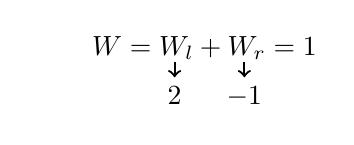
\begin{tikzpicture}[baseline=(base)]
                        \node (base) {$\quad \quad W = W_l + W_r = 1$};

                        \coordinate (Wl) at ([xshift=5.33em]base.base west);
                        \coordinate (Wr) at ([xshift=7.85em]base.base west);

                        % Labels
                        \node[below=1.8ex of Wl] (lval) {\normalsize 2};
                        \node[below=1.8ex of Wr] (rval) {\normalsize $-1$};

                        % Arrows pointing down from W_l and W_r
                        \draw[->, thick] ([yshift=-0.5ex]Wl) -- (lval.north);
                        \draw[->, thick] ([yshift=-0.5ex]Wr) -- (rval.north);
                    \end{tikzpicture}
                \] \\
                \vspace{-0.5em}
                {\large Configuration accepted, see (e), hence machine does not halt starting from $\texttt{10101}\; \texttt{\stateC}\sone\; \texttt{01}$, see Theorem~\ref{th:WFAR}. }
                }
                % \begin{tikzpicture}[->, >=Stealth, auto, node distance=2cm, every node/.style={scale=1}]
                %     \tikzset{
                %         state/.style={
                %                 circle, draw, minimum size=1cm, inner sep=1pt
                %             }
                %     }

                %     % % Upper isolated state
                %     % \node[state] (1top) at (0,2.5) {1};
                %     % \draw[->] (1top) edge[loop above] node{1} (1top);
                %     % \draw[->] (1top) edge[loop left] node{0} (1top);

                %     % Lower automaton
                %     \node[state] (0) at (0,0) {0};
                %     \node[state] (2) at (3,0) {1};

                %     \draw[->] (0) edge[loop above] node{0} (0);
                %     \draw[->] (2) edge[loop above] node{1} (2);

                %     \draw[->] (0) edge[bend left=10] node{1} (2);
                %     \draw[->, red, bend left=20, thick] (2) to node[below]{0} (0);

                %     % Initial state arrow
                %     \draw[->] (-1,0) -- (0);
                % \end{tikzpicture}
            \end{minipage}
        }

        \vspace{0.5em}
        \raggedright
        (e) Accepted weighted configurations \\
        \centering

        \usetikzlibrary{positioning, shapes.multipart, fit}
        \scalebox{0.8}{
            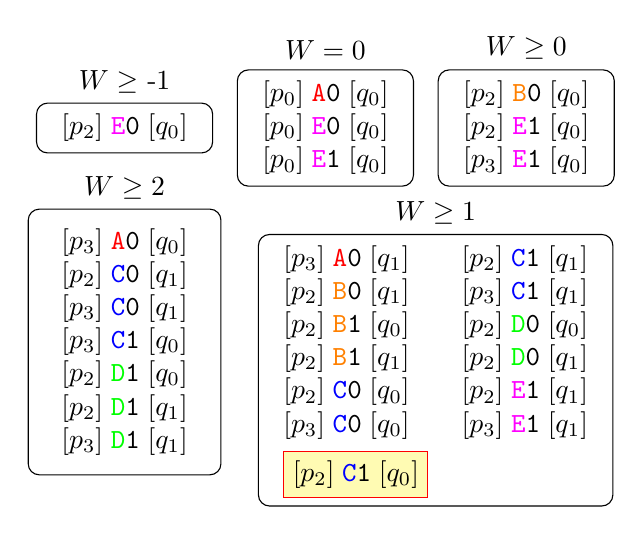
\begin{tikzpicture}[node distance=0.2cm and 0.3cm, every node/.style={font=\normalsize}, anchor=north]

                % Reference coordinate for top alignment
                \coordinate (topref) at (0,0);

                % W >= -1 group
                \node[draw, rectangle, rounded corners, inner sep=3pt] (wmin1box)
                {\begin{tabular}{l}
                        $[p_2]\; \texttt{\stateE}\szero\; [q_0]$
                    \end{tabular}};
                \node[above=0cm of wmin1box] {$W \geq$ -1};

                % W = 0 group
                \node[draw, rectangle, rounded corners, inner sep=3pt, right=of wmin1box] (w0box)
                {\begin{tabular}{l}
                        $[p_0]\; \texttt{\stateA}\szero\; [q_0]$ \\
                        $[p_0]\; \texttt{\stateE}\szero\; [q_0]$ \\
                        $[p_0]\; \texttt{\stateE}\sone\; [q_0]$
                    \end{tabular}};
                \node[above=0cm of w0box] {$W = 0$};

                % W >= 0 group
                \node[draw, rectangle, rounded corners, inner sep=3pt, right=of w0box] (w0plusbox)
                {\begin{tabular}{l}
                        $[p_2]\; \texttt{\stateB}\szero\; [q_0]$ \\
                        $[p_2]\; \texttt{\stateE}\sone\; [q_0]$  \\
                        $[p_3]\; \texttt{\stateE}\sone\; [q_0]$
                    \end{tabular}};
                \node[above=0cm of w0plusbox] {$W\geq0$};
                % W >= 1 group
                \node[draw, rectangle, rounded corners, inner sep=3pt, below=0.6cm of w0box, xshift=1.4cm] (w1box)
                {\begin{tabular}{ll}
                        $[p_3]\; \texttt{\stateA}\szero\; [q_1]$                                             & $[p_2]\; \texttt{\stateC}\sone\; [q_1]$  \\
                        $[p_2]\; \texttt{\stateB}\szero\; [q_1]$                                             & $[p_3]\; \texttt{\stateC}\sone\; [q_1]$  \\
                        $[p_2]\; \texttt{\stateB}\sone\; [q_0]$                                              & $[p_2]\; \texttt{\stateD}\szero\; [q_0]$ \\
                        $[p_2]\; \texttt{\stateB}\sone\; [q_1]$                                              & $[p_2]\; \texttt{\stateD}\szero\; [q_1]$ \\
                        $[p_2]\; \texttt{\stateC}\szero\; [q_0]$                                             & $[p_2]\; \texttt{\stateE}\sone\; [q_1]$  \\
                        $[p_3]\; \texttt{\stateC}\szero\; [q_0]$                                             & $[p_3]\; \texttt{\stateE}\sone\; [q_1]$  \\
                        \rule{0pt}{3.3ex}\fcolorbox{red}{yellow!30}{$[p_2]\; \texttt{\stateC}\sone\; [q_0]$} &                                          \\
                    \end{tabular}};
                \node[above=0cm of w1box] {$W \geq 1$};

                % W >= 2 group
                \node[draw, rectangle, rounded corners, inner sep=6pt, below=0.7cm of wmin1box] (w2box)
                {\begin{tabular}{l}
                        $[p_3]\; \texttt{\stateA}\szero\; [q_0]$ \\
                        $[p_2]\; \texttt{\stateC}\szero\; [q_1]$ \\
                        $[p_3]\; \texttt{\stateC}\szero\; [q_1]$ \\
                        $[p_3]\; \texttt{\stateC}\sone\; [q_0]$  \\
                        $[p_2]\; \texttt{\stateD}\sone\; [q_0]$  \\
                        $[p_2]\; \texttt{\stateD}\sone\; [q_1]$  \\
                        $[p_3]\; \texttt{\stateD}\sone\; [q_1]$  \\
                    \end{tabular}};
                \node[above=0cm of w2box] {$W \geq 2$};

            \end{tikzpicture}
        }
    \end{minipage}

    \caption{{\small WFAR certificate of nonhalting for machine \tm{1RB---_0RC1LC_1RD1RC_1LE1LD_0RA0LE}: (a) transition table and 20,000-step space-time diagram, (b) left weighted automaton: processes symbols to the left of the head in the left-to-right direction, which results in a left end-state -- \eg state $p_2$ when processing \texttt{10101} -- and a left weight obtained by summing the weights of each transition -- \eg $W_l = 2$ when processing \texttt{10101} (c) right weighted automaton: processes symbols to the right of the head (excluding the symbol read by the head) in the right-to-left direction -- indicated with arrow --, which results in a right end-state -- \eg state $q_0$ when processing \texttt{01} right-to-left -- and a right weight -- \eg $W_r = -1$ when processing \texttt{01} right-to-left (d) example, the total weight of configuration $\texttt{10101}\; \texttt{\stateC}\sone\; \texttt{01}$ is $W=W_l+W_r = 1$, using same word-encoding of configurations as in Section~\ref{sec:FAR}, and the right and left end-states are $p_2$ and $q_0$. Weighted automaton configuration $[p_2]\; \texttt{\stateC}\texttt{1}\; [q_0]$ with $W = 1$ is in the set of accepted weighted configurations (under more general $W \geq 1$), see (e). Therefore we know that the machine does not halt from configuration $\texttt{10101}\; \texttt{\stateC}\sone\; \texttt{01}$, Theorem~\ref{th:WFAR}. Similarly, Turing machine configuration $\texttt{\stateA}\texttt{0}$, which results in weighted configuration $[p_0]\;\texttt{\stateA}\texttt{0}\; [q_0]$ with $W=0$ is accepted, ensuring that the machine does not halt from the all-0 initial tape, Theorem~\ref{th:WFAR}.}}\label{fig:WFAR}
\end{figure}

\subsubsection{Overview}\label{sec:WFAR:overview}



\begin{figure}
    \centering
    \begin{tikzpicture}[->, >=Stealth, auto, node distance=2cm, every node/.style={scale=1}]
        \tikzset{
            state/.style={
                    circle, draw, minimum size=1cm, inner sep=1pt
                }
        }

        % % Upper isolated state
        % \node[state] (1top) at (0,2.5) {1};
        % \draw[->] (1top) edge[loop above] node{1} (1top);
        % \draw[->] (1top) edge[loop left] node{0} (1top);

        % Lower automaton
        \node[state] (0) at (0,0) {$q_0$};
        \node[state] (2) at (3,0) {$q_1$};
        \node[state] (3) at (6,0) {$q_2$};

        \draw[->, green!70!black, thick] (0) edge[loop above] node{\szero} (0);
        \draw[->, red, thick] (2) edge[loop above] node{\sone} (2);
        \draw[->] (3) edge[loop above] node{\szero,\sone} (3);

        \draw[->, red, thick] (0) edge[bend left=10] node{\sone} (2);
        \draw[->] (2) to node[below]{\szero} (3);

        % Initial state arrow
        \draw[->] (-1,0) -- (0);

        % Compact and aligned legend
        \node[draw, right=0.5cm of 3, inner sep=3pt, rounded corners] (legend) {
            \scalebox{0.7}{
                \begin{tabular}{@{}rl@{}}
                    \tikz[baseline=-0.5ex]\draw[->, black, thick] (0,0) -- +(0.6,0);          & \;Weight 0    \\
                    \tikz[baseline=-0.5ex]\draw[->, green!70!black, thick] (0,0) -- +(0.6,0); & \;Weight 1    \\
                    \tikz[baseline=-0.5ex]\draw[->, red, thick] (0,0) -- +(0.6,0);            & \;Weight $-1$
                \end{tabular}
            }
        };
    \end{tikzpicture}
    \caption{Weighted automaton recognising nonregular language $\texttt{0}^n \texttt{1}^n$, using accept set $\{(q_1,W=0)\}$ or $\{(q_1,W=0), (q_0,W=0)\}$ if we include the empty word.}\label{fig:ex_wa}
\end{figure}

Weighted automata are an extension of usual finite state automata where each transition is given a weight in $\Z$: when a word is processed, total weight $W \in \Z$ is computed by summing the weights of all the encountered transitions. Accepted words are described by a set of pairs of final-state and weigth lower and upper bounds (potentially infinite) to satisfy: for instance, the archetypal nonregular language $\texttt{0}^n \texttt{1}^n$ is recognised by the weighted automaton of Figure~\ref{fig:ex_wa} using accept set $\{(q_1,0 \leq W \leq 0)\}$ which we can simplify as $\{(q_1,W=0)\}$ and we may add $(q_0,W=0)$ to the set if we want to include the empty word.

Weighted Finite Automata Reduction (WFAR) is an extension of FAR (Section~\ref{sec:FAR}) using deterministic weighted finite automata. Figure~\ref{fig:WFAR} gives a \textit{WFAR automaton}, which is a certificate of nonhalting the machine given in Figure~\ref{fig:WFAR}~(a). A WFAR automaton consists of (i) a \textit{left deterministic weighted automaton} (ii) a \textit{right deterministic weighted automaton} and (iii) a set of accepted \textit{weighted configurations}, see Figure~\ref{fig:WFAR}~(b), (c), and (e).
A WFAR automaton processes word-representations (as defined in Section~\ref{sec:FAR}) of Turing machine configurations\footnote{With finitely many $\sone$s, which we always assume from now on.} in the way describe below, and, if a configuration is accepted by the WFAR automaton, we know that the associated Turing machine does not halt from that configuration, Theorem~\ref{th:WFAR}. That way, WFAR is a CTL method (instead of co-CTL for FAR), see Section~\ref{sec:deciders-overview}. The WFAR automaton of Figure~\ref{fig:WFAR} accepts (see below for what it means) the initial configuration $\texttt{\stateA}\szero$, giving a certificate of nonhalting for the machine of Figure~\ref{fig:WFAR}~(a) from the all-0 tape.

The method was initially developed by Iijil as a decider \cite{iijil1_2025_14914502} and integrated to \CoqBB by mxdys as a verifier: similarly to FAR (Section~\ref{sec:FAR}), 17 WFAR certificates are directly hardcoded in the \Coq proof, see file \texttt{Verifier\_WFAR\_Hardcoded\_Certificates.v}, see Section~\ref{sec:WFAR:results} for results.

\paragraph{WFAR processing.} Let's describe how a WFAR automaton processes a word-represented Turing machine configuration in order to decider whether it is accepted or not, as illustrated in Figure~\ref{fig:WFAR}. WFAR is an extension of the ``Meet-in-the-middle''\footnote{See Section 6.6 in \cite{bbchallenge_part1}.} instance of FAR \cite{bbchallenge_part1}: word-representations of configurations are split into three segments, (i) word to the left of the head, (ii) head state and symbol, (iii) word to the right of the head; \eg $\texttt{10101}\; \texttt{\stateC}\sone\; \texttt{01}$, Figure~\ref{fig:WFAR}~(d). The left word -- here $\texttt{10101}$ -- is processed left-to-right by the left weighted automaton, Figure~\ref{fig:WFAR}~(b), and the right word -- here $\texttt{01}$ -- is processed right-to-left, by the right weighted automaton, Figure~\ref{fig:WFAR}~(c). In this case, this results in final left state $p_2$, final right state $q_0$, final left weight $W_l = 2$ and final right weight $W_r = -1$; the final total weight is $W = W_l + W_r = 1$, Figure~\ref{fig:WFAR}~(d). We denote this final \textit{weighted configuration} as $[p_2]\; \texttt{\stateC}\sone\; [q_0]$ with $W=1$. This final weighted configuration belongs to the set of accepted weighted configurations, Figure~\ref{fig:WFAR}~(e), which means that configuration $\texttt{10101}\; \texttt{\stateC}\sone\; \texttt{01}$ is \textit{accepted} by this WFAR automaton.


\subsubsection{WFAR theorem}

WFAR is CTL technique -- see Section~\ref{sec:deciders-overview}: a WFAR automaton for a given Turing machine is meant to recognise a language of configurations $\mathcal{L}$ that includes the initial all-0 configuration, closed under Turing machine steps and that does not contain any halting configuration. Hence, we get the following CTL formalism, plus leading/trailing zeros conditions similarly to FAR:
\begin{align}
    u \in \mathcal{L}                               & \iff 0u \in \mathcal{L}               &  & \text{(leading zeros ignored)}
    \tag{\ref{eq:lzignore}}
    \\
    u \in \mathcal{L}                               & \iff u0 \in \mathcal{L}               &  & \text{(trailing zeros ignored)}
    \tag{\ref{eq:tzignore}}
    \\
    c\TMstep\bot                                    & \implies \hat{c} \not \in \mathcal{L} &  & \text{(reject halt)} \label{eq:rejecthalt}     \\
    (c_1\TMstep c_2)\land \hat{c}_1 \in \mathcal{L} & \implies\hat{c}_2 \in \mathcal{L}     &  & \text{(forward closure)} \label{eq:forwardclo}
\end{align}

Let's now show how to verify that a given WFAR automaton for a given Turing machine $\mathcal{M}$ accepts such $\mathcal{L}$, hence providing a certificate that $\mathcal{M}$ does not halt from the all-0 tape.

In the following, $\delta_L: Q_L \times \balphabet \to Q_L$ and $\delta_R: Q_R \times \balphabet \to Q_R$ respectively refer to the transition functions of the deterministic left and right weighted automaton of a WFAR automaton, \eg Figure~\ref{fig:WFAR}~(b) and (c), with $Q_L = \{p_0, \, \dots, \, p_{n_L-1}\}$ and $Q_R = \{q_0, \, \dots, \, q_{n_R-1}\}$ their respective set of states with $n_L$ and $n_R$ the number of left/right states and $p_0$ and $q_0$ are the respective initial states of the left and right weighted automaton. Weights are given by $w_L: Q_L \times \balphabet \to \Z$ and $w_R: Q_R \times \balphabet \to \Z$. We write $\delta_\mathcal{M}:\states \times \balphabet \hookrightarrow \balphabet \times \{\text{L},\text{R}\} \times \states$ for the transition function of $\mathcal{M}$\footnote{In the following, we limit ourselves to the binary tape alphabet $\balphabet$, but the results generalise transparently to arbitrary alphabets $\alphabet$.}.

\paragraph{Leading/trailing zeros.} Checking Conditions~\eqref{eq:lzignore} and \eqref{eq:tzignore} for a WFAR automaton is simple: thanks to the left-to-right and right-to-left respective read directions for the left and right weighted automaton, we simply have to check that $\delta_L(p_0,\szero) = p_0$ and $\delta_R(q_0,\szero) = q_0$ as well as $w_L(p_0,\szero) = w_R(q_0,\szero) = 0$ to ensure the convention that the weight of all word-representations of the initial all-0 configuration is 0.

\paragraph{Forward closure, without weights: back to FAR.} First, let's reformulate forward closure for a WFAR automaton, ignoring weights computations. Forward closure concerns the WFAR automaton's accept state, let's consider an example first. The WFAR automaton of Figure~\ref{fig:WFAR} accepts the initial Turing machine configuration $\texttt{\stateA}\szero$: the WFAR configuration $[p_0] \; \texttt{\stateA}\szero\; [q_0]$ (ignoring $W=0$) is in the accept set given in Figure~\ref{fig:WFAR}~(e). To ensure forward closure, Condition~\ref{eq:forwardclo}, let's consider how $\delta_\mathcal{M}(\texttt{\stateA},\szero) = \texttt{1R\stateB}$ affects $[p_0] \; \texttt{\stateA}\szero\; [q_0]$; we get $[p_0] \; \texttt{1}\; \texttt{\stateB}\texttt{?}\; [\texttt{?}]$, which is $[p_2] \; \texttt{\stateB}\texttt{?}\; [\texttt{?}]$ given that $\delta_L(p_0,\sone) = p_2$, see Figure~\ref{fig:WFAR}~(b). In order to resolve $\texttt{?}$, we look at all the transitions in the right weighted automaton that lead to $q_0$, see Figure~\ref{fig:WFAR}~(c): there are two, both reading a \texttt{0}, giving $[p_2] \; \texttt{\stateB}\texttt{0}\; [q_0]$ and $[p_2] \; \texttt{\stateB}\texttt{0}\; [q_1]$. Ignoring weights, we want both in the accept set:\footnote{Which is the case here, with $W\geq 0$ and $W \geq 1$ in Figure~\ref{fig:WFAR}~(e).} that ensures that for any Turing machine configuration $c_1$ yielding WFAR configuration $[p_0] \; \texttt{\stateA}\szero\; [q_0]$, then $c_2$ is also accepted by the WFAR automaton with $c_1 \TMstep c_2$. Note that $c_1$ and $c_2$ are not necessarily reachable from the initial all-0 tape: CTL methods provide languages that over-estimate the language generated by Turing machines from the all-0 tape.

In general, ignoring weights, forward closure means the following for WFAR automaton accept set $\mathfrak{A}$:
\begin{align}
     & \forall q', r' \in Q_R \times \balphabet \text{ s.t. } \delta_R(q', r') = q,
     &                                                                              & [p]\, fr\, [q] \in \mathfrak{A} \Rightarrow [\delta_L(p,b)]\, tr'\, [q'] \in \mathfrak{A}
     &                                                                              & \text{if } \delta_{\mathcal{M}}(f,r) = (b, \text{R}, t) \label{eq:forwardcloR}
    \\[0.5em]
     & \forall p', r' \in Q_L\times \balphabet \text{ s.t. } \delta_L(p', r') = p,
     &                                                                              & [p]\, fr\, [q] \in \mathfrak{A} \Rightarrow [p']\, tr'\, [\delta_R(q,b)] \in \mathfrak{A}
     &                                                                              & \text{if } \delta_{\mathcal{M}}(f,r) = (b, \text{L}, t) \label{eq:forwardcloL}
\end{align}

For all left/right weighted automata states $p,q \in Q_L \times Q_R$ and notations $f,t \in \{\stateA,\stateB,\stateC,\stateD,\stateE\}$ the ``from'' and ``to'' states in a transition, $r,b \in \balphabet$ respectively the bit read and the bit written in a transition. If, ignoring weights, a WFAR accept set is forward-closed in the above sense, contains no halting configuration, and contains $[p_0] \; \texttt{\stateA}\szero\; [q_0]$, then we are in a particular case of FAR, as shown in \cite{bbchallenge_part1} \ie Theorem~\ref{far-main-theorem} can be applied: the Turing machine does not halt from the initial all-0 configuration and, is regular in the sense of Section~\ref{sec:deciders-overview}.

\paragraph{Forward closure, with weights: beyond FAR.} Weights allow to further restrict the accept set in cases where the above, \textit{weight-less}, forward closure does include halting configurations. For instance, in the case of Figure~\ref{fig:WFAR}, we have $[p_2] \; \texttt{\stateD}\sone \; [q_1]$ (with $W \geq 2$) in the accept set $\mathfrak{A}$, given in Figure~\ref{fig:WFAR}~(e), and, computing weight-less forward closure from this WFAR configuration, ignoring weights, yields, using \eqref{eq:forwardcloR} and, \eqref{eq:forwardcloL}, $[p_0] \; \texttt{\stateD}\sone \; [q_1]$, then $[p_0] \; \texttt{\stateD}\szero \; [q_1]$, then $[p_0] \; \texttt{\stateE}\szero \; [q_1]$ and finally, $[p_0] \; \texttt{\stateA}\sone \; [q_0] $, which is a halting configuration, meaning that we cannot conclude that $\mathcal{M}$ does not halt from the initial all-0 configuration. However, looking at Figure~\ref{fig:WFAR}~(e) we see that $[p_0] \; \texttt{\stateD}\sone \; [q_1] \not \in \mathfrak{A}$ and hence none of the successors either. This \textit{refinement} of $\mathfrak{A}$ is due to discarding \textit{impossible} weighted configurations, which we explain now.

With weights, WFAR configurations are expressed as follows: $[p] \; fr \; [q];\; W \geq m; \; W \leq M;$ with $m \in \Z \cup\{-\infty\}$ and $M \in \Z \cup \{+\infty\}$ weights bounds. For instance, considering the accept state $\mathfrak{A}$ of Figure~\ref{fig:WFAR}~(e) with weights, we have that the initial weighted configuration, $c'_1 = [p_0] \; \texttt{\stateA}\szero \; [q_0];\; W \geq 0;\; W \leq 0;$ is in $\mathfrak{A}$. When computing closure, bounds are updated by the \textit{total weight change} incurred when processing weighted transitions: consider $c'_2 = [p_2] \; \texttt{\stateB}\szero \; [q_1];\; W \geq \texttt{?};\; W \leq \texttt{?}$ obtained from the initial weighted configuration by \eqref{eq:forwardcloR}; we have $W(c_2) = W(c_1) + w_L(p_0,\sone) - w_R(q_1, \szero)$ with $c_1 \TMstep c_2$ Turing machine configurations such that $c_1$ yields WFAR configuration $c'_1$ and $c_2$ yields $c'_2$. Hence, for $c'_2$ to be accepted, we must update its weight bounds by weight change $w_L(p_0,\sone) - w_R(q_1, \szero) = 0 - (- 1) = +1$, giving $c'_2 = [p_2] \; \texttt{\stateB}\szero \; [q_1];\; W \geq 1;\; W \leq 1$, which is implied by more general $c'_2 = [p_2] \; \texttt{\stateB}\szero \; [q_1];\; W \geq 1;\; W < +\infty$ in $\mathfrak{A}$ of Figure~\ref{fig:WFAR}~(e). In general, in the case of \eqref{eq:forwardcloR}, using same notations, weights bounds $m$ and $M$ are added to weight change $w_L(p,b) - w_R(q', r')$ and weight change $w_L(p',r') - w_R(q,b)$ in the case of \eqref{eq:forwardcloL}; infinite bounds remain the same under any weight change.

Coming back to $[p_2] \; \texttt{\stateD}\sone \; [q_1];\; W \geq 2;\; W \leq + \infty;$ which we have shown above to lead to a halting configuration, we can now compute the bounds of the weighted configuration we obtained using \eqref{eq:forwardcloL}: $[p_0] \; \texttt{\stateD}\sone \; [q_1]\; W \geq 2; \; W < +\infty;$ as there is no weight changes. However, note that any left word reaching $q_0$ has left weight $W_l = 0$ and any right word reaching $q_1$ has right weight $W_r \leq 0$, hence total weight $W \leq 0$, which is incompatible with the constraint $W \geq 2$; hence we can discard $[p_0] \; \texttt{\stateD}\sone \; [q_1]\; W \geq 2; \; W < +\infty$ from the accept set $\mathfrak{A}$ as it is an impossible weighted configuration. Doing this also discards from $\mathfrak{A}$ all the weighted configurations we computed from $[p_0] \; \texttt{\stateD}\sone \; [q_1]\; W \geq 2; \; W < +\infty$, including the halting one, $[p_0] \; \texttt{\stateA}\sone \; [q_0] $.

In this case, in order to conclude, we needed to know that, in the left weighted automaton of Figure~\ref{fig:WFAR}~(b), terminating at state $q_0$ implies $W_l = 0$. In general, the exact feasible weight bounds of any state in a weighted automaton can be computed using the Bellman-Ford algorithm\footnote{Using Bellman-Ford was suggested by a LLM. However both the original and the \CoqBB implementations do not need it as they use restricted weighted automata on which it is easy to check whether the feasible weights for each state are nonpositive or nonnegative \cite{iijil1_2025_14914502}.}: for instance, in the left weighted automaton of Figure~\ref{fig:WFAR}~(b), at state $p_2$, we have $0 \leq W_l < +\infty$. Hence we can use these feasible weight bounds to automatically discard impossible weighted configurations from $\mathfrak{A}$ and hopefully, end up with no halting configuration in $\mathfrak{A}$.

We say that $\mathfrak{A}$ is \textit{weighted forward closed}\tsm{Iijil commented that this definition \href{https://discord.com/channels/960643023006490684/1151558585344593950/1365426047176151080}{needs improvement}.} for machine $\mathcal{M}$ if (i) for all weighted configuration $c \in \mathfrak{A}$, for any weighted configurations $c'$ obtained by closure using \eqref{eq:forwardcloL} or \eqref{eq:forwardcloR} together with the weights bounds update rules stated above, there is $c'' \in \mathfrak{A}$ with bounds $m''$ and $M''$ such that $m'' \leq m'$ and $M'' \geq M'$ with $m'$ and $M'$ the bounds of $c'$ and (ii) there is no impossible weighted configuration in $\mathcal{A}$ as defined above, \ie incompatible with the feasible weight bounds computed from the left and right weighted automata.

We finally get the WFAR theorem:

\begin{theorem}[\CoqBB: \texttt{Lemma MITM\_WDFA\_verifier\_spec}]\label{th:WFAR}
    Let $\mathcal{M}$ be a Turing machines and $\mathcal{W}$ be a WFAR automaton with accept set $\mathfrak{A}$ such that:
    \begin{enumerate}
        \item Leading and trailing zeros are ignored: $\delta_L(p_0,\szero) = p_0$ and $\delta_R(q_0,\szero) = q_0$ with $w_L(p_0,\szero) = w_R(q_0,\szero) = 0$ with $\delta_L$ and $\delta_R$ the transition functions of the left and right weighted automata of $\mathcal{W}$ and $w_L$ and $w_R$ their weighing functions.\label{pt:wfar:top}
        \item The initial configuration is accepted: \ie $[p_0]\; \texttt{\stateA}\szero\; [q_0];\; W=0;$ is in $\mathfrak{A}$.\label{pt:wfar:ttop}
        \item $\mathfrak{A}$ is weighted forward closed for $\mathcal{M}$.\label{pt:wfar:tttop}
        \item $\mathfrak{A}$ contains no halting configurations.\label{pt:wfar:ttttop}
    \end{enumerate}

    Then $\mathcal{M}$ does not halt for any configuration accepted by $\mathcal{W}$, which includes the initial all-0 configuration.
\end{theorem}
\begin{proof}
    Point~\ref{pt:wfar:top} guarantees that all the word-representations (see Section~\ref{sec:FAR}) of the same Turing machine configurations result in the same weighted WFAR configuration when processed by $\mathcal{W}$ (see Section~\ref{sec:WFAR:overview}). Points \ref{pt:wfar:ttop}-\ref{pt:wfar:ttttop} are the WFAR reformulations of the CTL argument (Section~\ref{sec:deciders-overview}). Hence, using the CTL argument, any Turing machine configuration accepted by $\mathcal{W}$ is nonhalting, and, in particular, the initial all-0 configuration.
\end{proof}





\subsubsection{Implementations and results}\label{sec:WFAR:results}

\CoqBB implements Theorem~\ref{th:WFAR}, see file \texttt{Verifier\_WFAR.v}. Certificates consist of left and right weighted automaton: accept sets are constructed by the \Coq verifier which computes the closure from $[p_0]\; \texttt{\stateA} \szero\; [q_0]; W=0$ and uses an integer parameter $P$ given in the certificate such that a bound $W \geq P$ is replaced by $W \leq +\infty$. See the 17 certificates in \texttt{Verifier\_WFAR\_Hardcoded\_Certificates.v}.

These certificates were mainly found by the original WFAR decider implementation \cite{iijil1_2025_14914502} which searches the space of WFAs using bruteforce. Certificates for ``Helices'' (see Section~\ref{sec:WFAR}) were handcrafted by Blanchard and are significantly bigger than the other certificates: about 50 states in the left and right WAs each where other certificates have less than 10 in each.

\newpage
\section{Sporadic 5-state machines}\label{sec:sporadic}

\newpage
\section{Results}\label{sec:sporadic}

\newpage
\section{Zoology}\label{sec:sporadic}


\bibliographystyle{abbrv}
\newpage
\bibliography{bbchallenge-paper}

\appendix


\section{Busy Beavers lower bounds}\label{app:lowerbounds}
\section{Exact pipelines}\label{app:pipelines}
\section{Cryptids}\label{app:cryptids}

\end{document}
